\documentclass[10pt]{article}
%%%%%%%%%%%%%%%%%%%%%%%%%
%			AZ' STANDARD NEWCOMMANDS
%%%%%%%%%%%%%%%%%%%%%%%%%
\usepackage[applemac]{inputenc}
\usepackage[english]{babel}
\usepackage[T1]{fontenc}
\usepackage{cite, url,color} % Citation numbers being automatically sorted and properly "compressed/ranged".
%\usepackage{pgfplots}
\usepackage{graphics,amsfonts}
\usepackage[pdftex]{graphicx}
\usepackage[cmex10]{amsmath}
% Also, note that the amsmath package sets \interdisplaylinepenalty to 10000
% thus preventing page breaks from occurring within multiline equations. Use:
 \interdisplaylinepenalty=2500
% after loading amsmath to restore such page breaks as IEEEtran.cls normally does.

%% Useful packages for creation of two-column and more complex figures
% Compact lists
\usepackage{enumitem}
\usepackage{booktabs}
\usepackage{fancyvrb}

\usepackage{listings} % inserisce listati di programmi
\definecolor{commenti}{rgb}{0.13,0.55,0.13}
\definecolor{stringhe}{rgb}{0.63,0.125,0.94}
\lstloadlanguages{Matlab}
\lstset{% general command to set parameter(s)
framexleftmargin=0mm,
frame=single,
keywordstyle = \color{blue},% blue keywords
identifierstyle =, % nothing happens
commentstyle = \color{commenti}, % comments
stringstyle = \ttfamily \color{stringhe}, % typewriter type for strings
showstringspaces = false, % no special string spaces
emph = {for, if, then, else, end},
emphstyle = \color{blue},
firstnumber = 1, % numero della prima linea
numbers =right, %  show number_line
numberstyle = \tiny, % style of number_line
stepnumber = 5, % one number_line after stepnumber
numbersep = 5pt,
language = {Matlab}, % per riconoscere la sintassi matlab
extendedchars = true, % per abilitare caratteri particolari
breaklines = true, % per mandare a capo le righe troppo lunghe
breakautoindent = true, % indenta le righe spezzate
breakindent = 30pt, % indenta le righe di 30pt
basicstyle=\footnotesize\ttfamily
}

\usepackage{array}
% http://www.ctan.org/tex-archive/macros/latex/required/tools/
\usepackage{mdwmath}
\usepackage{mdwtab}
%mdwtab.sty	-- A complete ground-up rewrite of LaTeX's `tabular' and  `array' environments.  Has lots of advantages over
%		   the standard version, and over the version in `array.sty'.
% *** SUBFIGURE PACKAGES ***
\usepackage[tight,footnotesize]{subfigure}

\usepackage[top=2cm, bottom=2cm, right=1.6cm,left=1.6cm]{geometry}
\usepackage{indentfirst}

%\usepackage{times}
%\usepackage[active]{srcltx}
\graphicspath{{./figure/}}

\setlength\parindent{0pt}
\linespread{1}

\def\C#1{\mathcal{#1}}

\usepackage{mathtools}
\DeclarePairedDelimiter{\ceil}{\lceil}{\rceil}
\DeclarePairedDelimiter{\floor}{\lfloor}{\rfloor}

% Package used to keep inherent figures in the same section
\usepackage{placeins}


\begin{document}
\title{Network Analysis and Simulation - Homework 1}
\author{Michele Polese, 1100877}

\maketitle

\section{Estimators}
The following MATLAB code describes the estimators used in all the scripts of this homework. They are written as functions for code reusability.
\subsubsection*{Estimator for q-quantiles}
The q-quantile estimator of a dataset \{$x_1, ... , x_n$\} is defined as $\frac{x_{(j)}+x_{(k)}}{2}$ with \{$x_{(1)}^n, ... , x_{(n)}^n$\} the order statistic, $j = \floor{qn + (1 - q)}$, $j = \ceil{qn + (1 - q)}$.
\lstinputlisting{../code/qquant_est.m}

\subsubsection*{Estimator for the mean}
The sample mean over a dataset \{$x_1, ... , x_n$\} is defined as $\hat{\mu}_n = \frac{1}{n}\sum_{i=1}^n x_i$.
\lstinputlisting{../code/mean_est.m}

\subsubsection*{Estimator for the variance}
The sample variance over a dataset \{$x_1, ... , x_n$\} is defined as $\hat{s}_n^2 = \frac{1}{n - 1}\sum_{i=1}^n (x_i - \hat{\mu}_n)^2$ (unbiased estimator) or $\hat{s}_n^2 = \frac{1}{n}\sum_{i=1}^n (x_i - \hat{\mu}_n)^2$ (biased estimator).
\lstinputlisting{../code/var_est.m}

\subsubsection*{Estimator for the autocorrelation}
Biased estimator for autocorrelation can be found in \cite{leb}. Given the dataset \{$x_1, ... , x_n$\} the sample autocorrelation sequence (ACS) is $\hat{\rho}_t = \hat{\gamma}_t / \hat{\gamma}_0$, with $\hat{\gamma}_t$ the sample autocovariance $\hat{\gamma}_t = \frac{1}{n}\sum_{s=1}^{n-t} (x_{s + t} - \hat{\mu}_n)(x_{s} - \hat{\mu}_n)$ ($\hat{\mu}_n$ is the sample mean).
\lstinputlisting{../code/autocorrelation.m}

\section{Exercise 1}
The following Figures contain plots from Figures 2.1, 2.2, 2.3, 2.7, 2.8 and 2.10 in \cite{leb}. In Figure~\ref{fig:22} there is a plot of the empirical cumulative distribution function for the two dataset. Given a dataset \{$x_1, ... , x_n$\} the ECDF is defined as $F(x)=\frac{1}{n}\sum_{i=1}^n1_{x_i \le x}$.


\begin{figure}[h!]
  \centering
  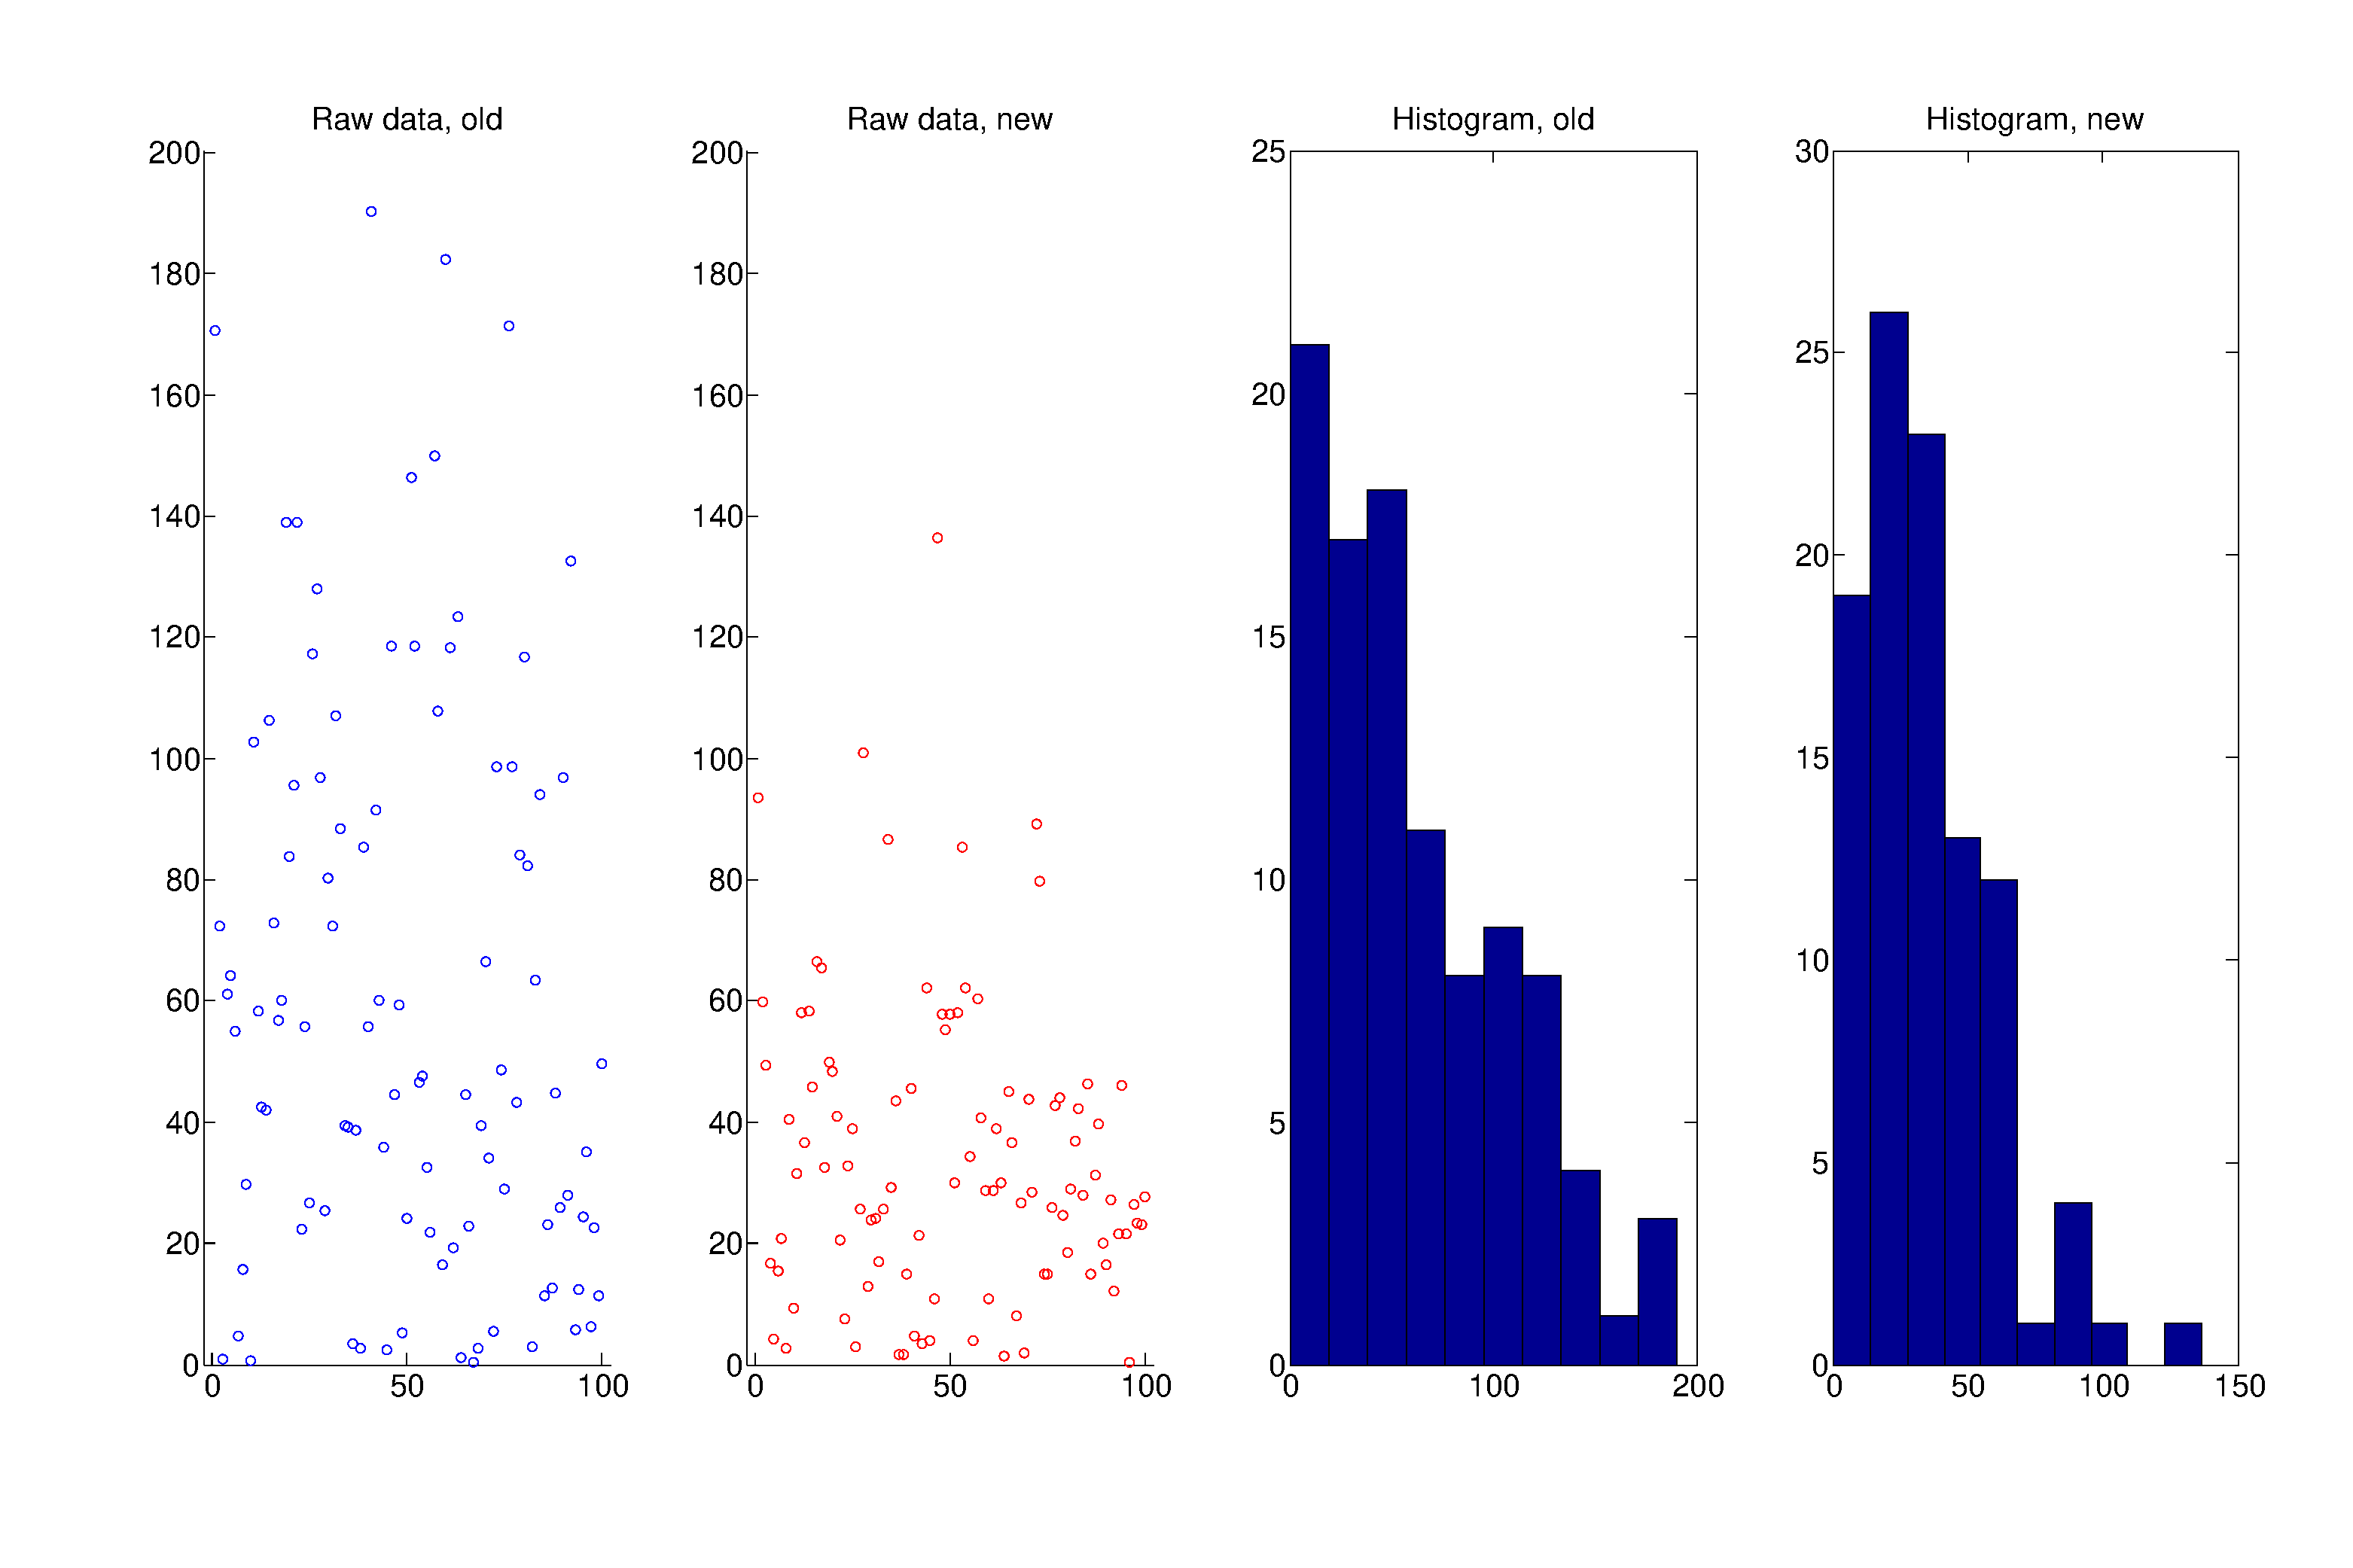
\includegraphics[width=0.8\textwidth]{images/hw1_1_21}
  \caption{Figure 2.1 in \cite{leb}. Different way to compare two datasets.}
  \label{fig:21}
\end{figure}


\begin{figure}[h!]
  \centering
  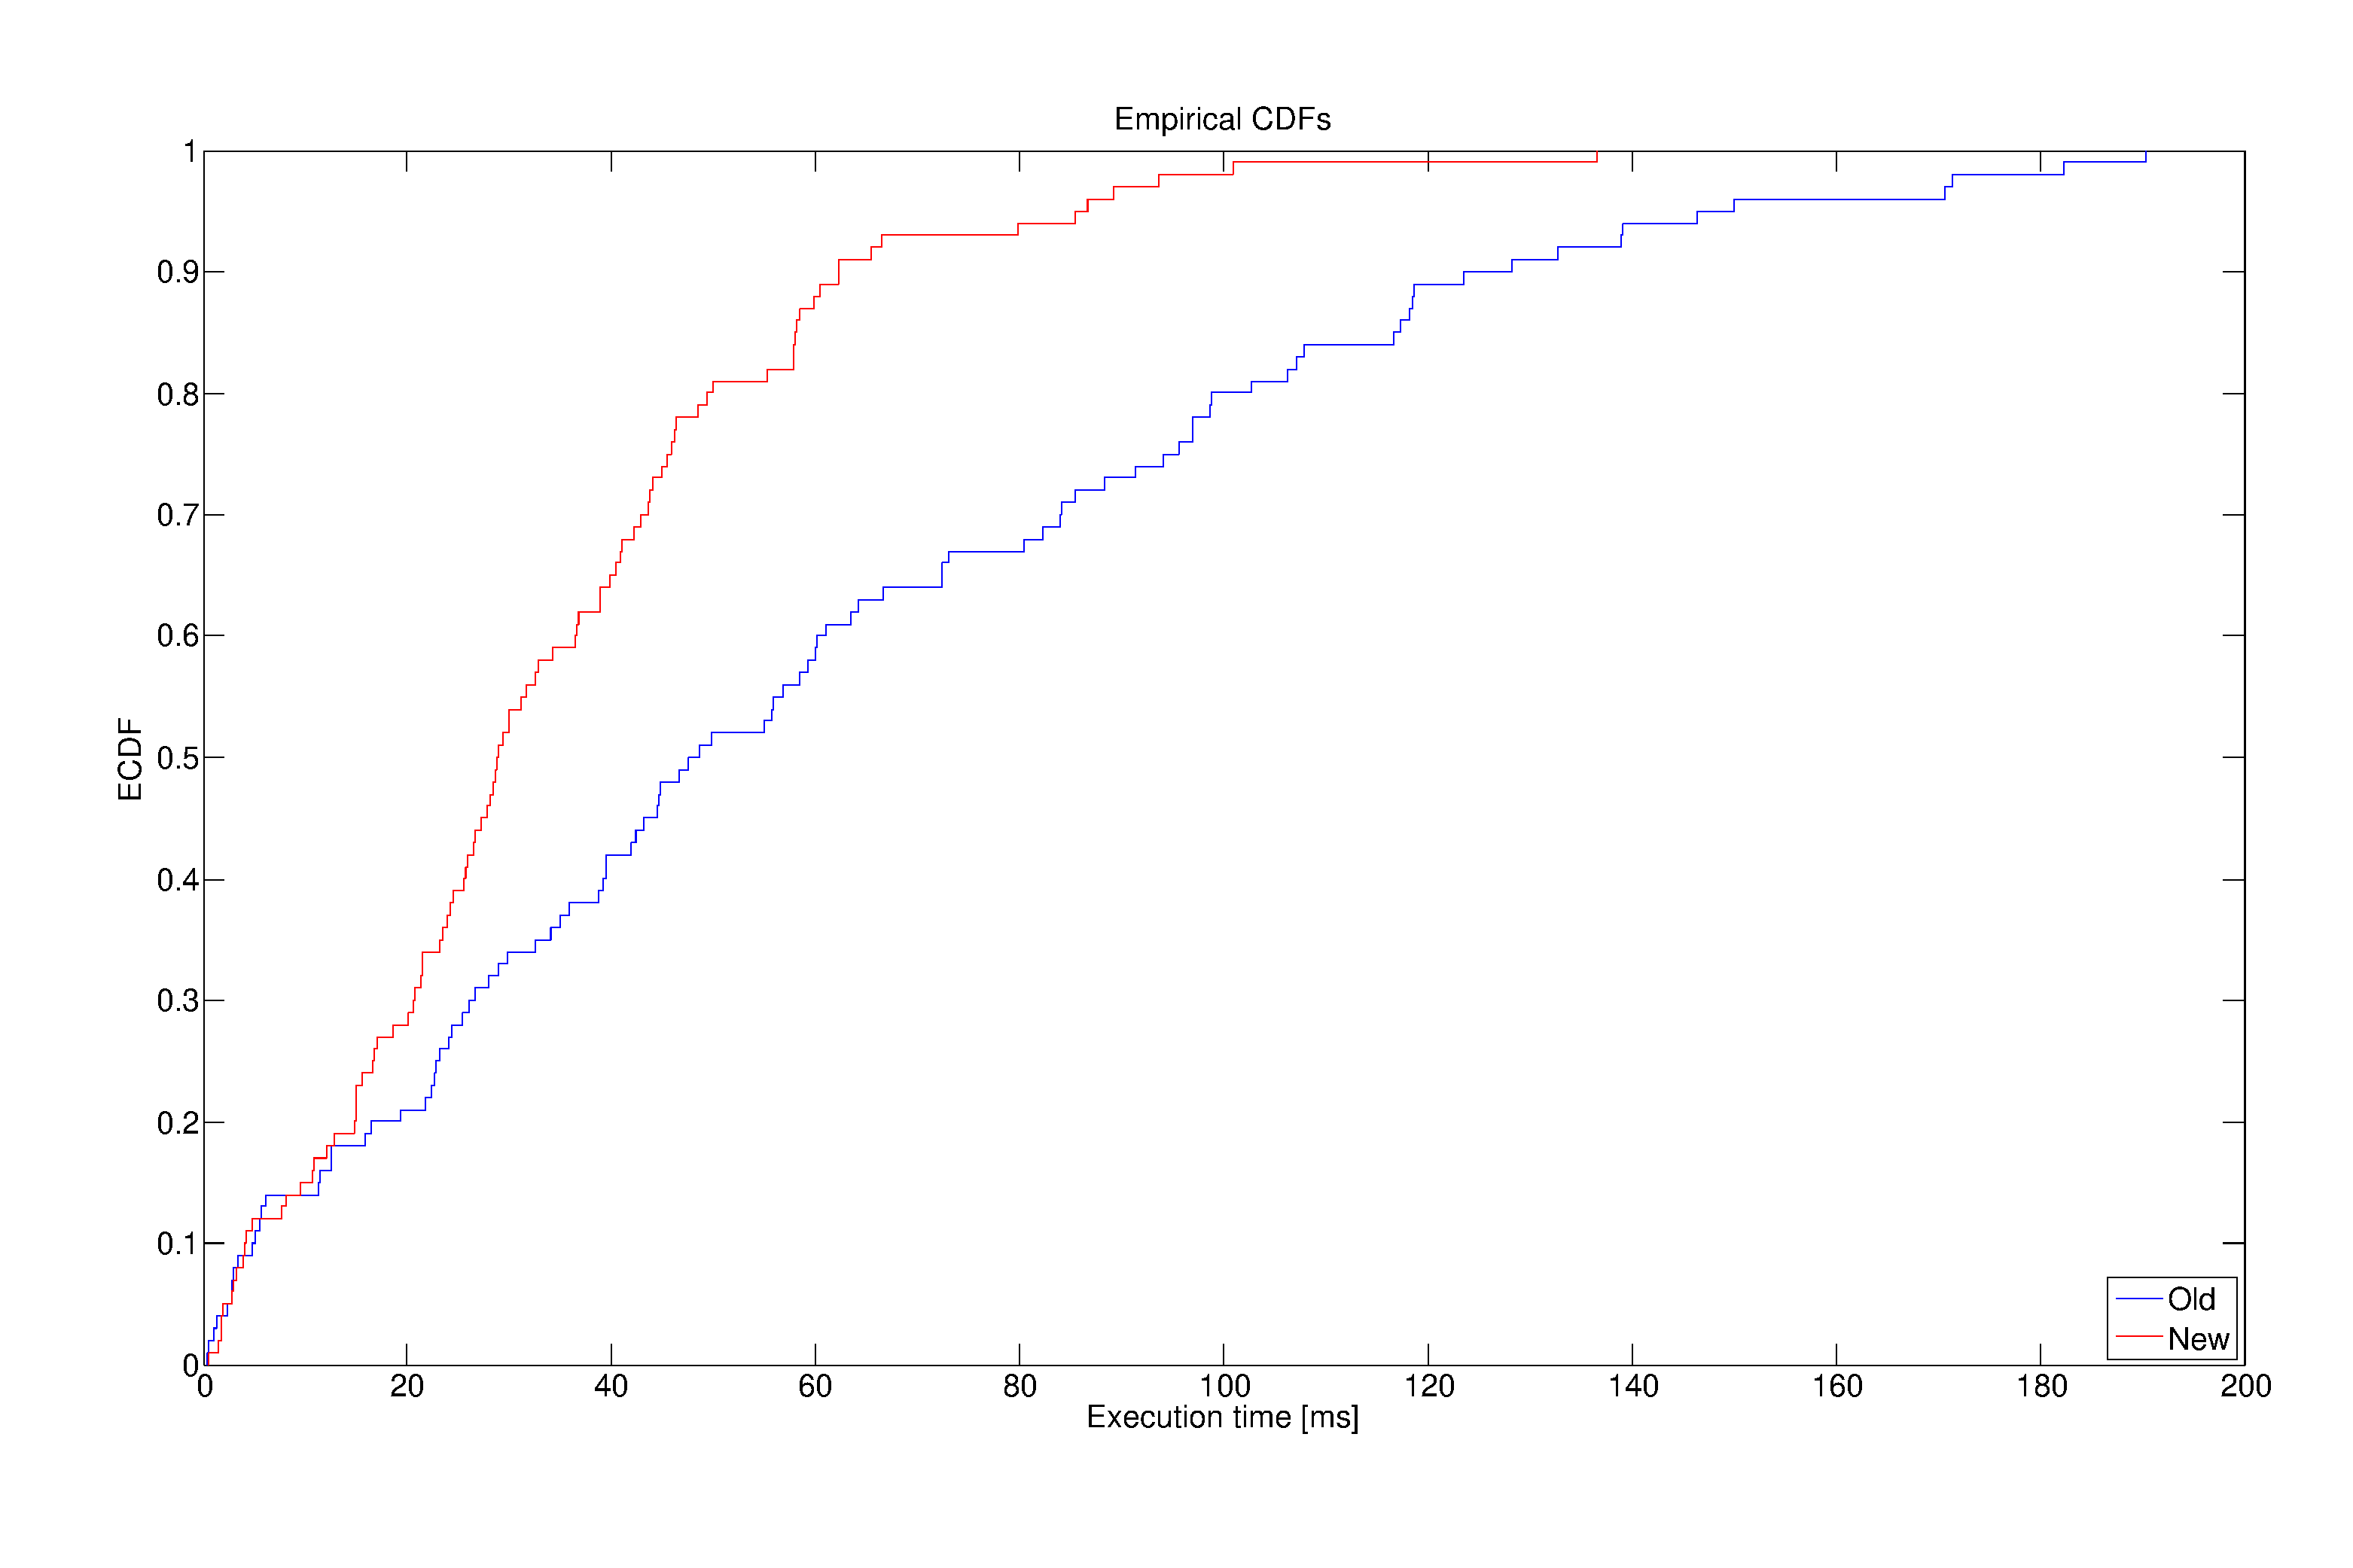
\includegraphics[width=0.7\textwidth]{images/hw1_1_22}
  \caption{Figure 2.2 in \cite{leb}. Empirical CDF for the 2 datasets.}
  \label{fig:22}
\end{figure}

\begin{figure}[h!]
  \centering
  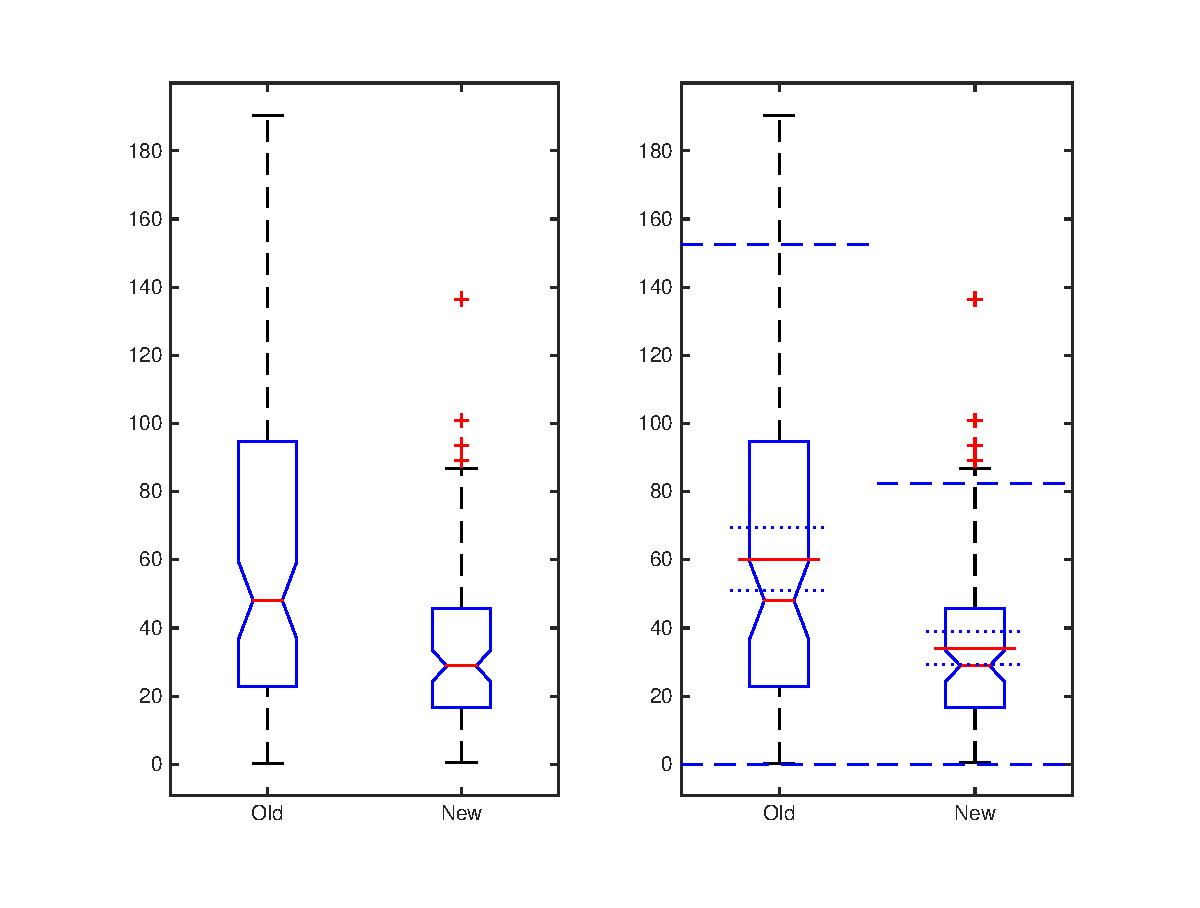
\includegraphics[width=0.7\textwidth]{images/hw1_1_23}
  \caption{Figure 2.3 in \cite{leb}. Boxplots.}
  \label{fig:23}
\end{figure}

\begin{figure}[h!]
  \centering
  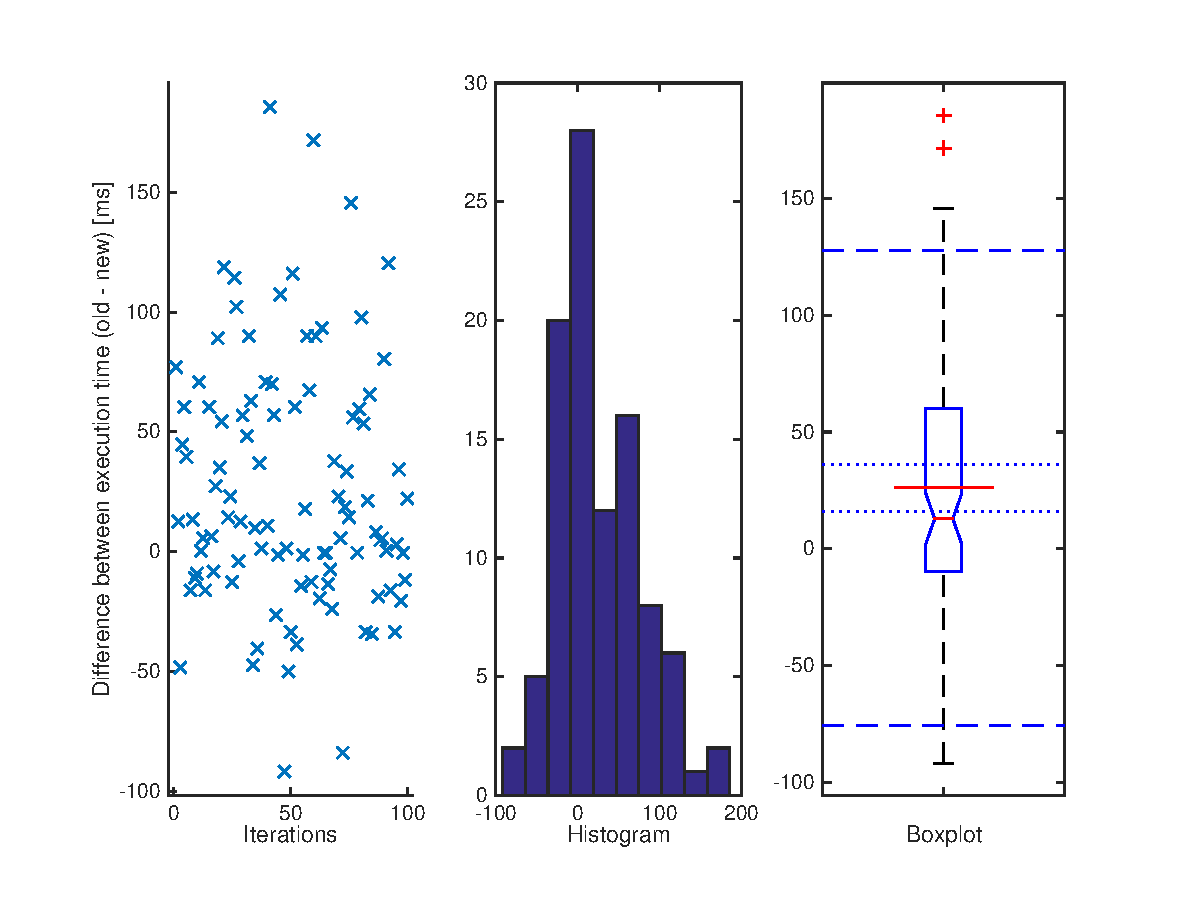
\includegraphics[width=0.7\textwidth]{images/hw1_1_27}
  \caption{Figure 2.7 in \cite{leb}. Difference between the 2 datasets.}
  \label{fig:27}
\end{figure}

\begin{figure}[h!]
  \centering
  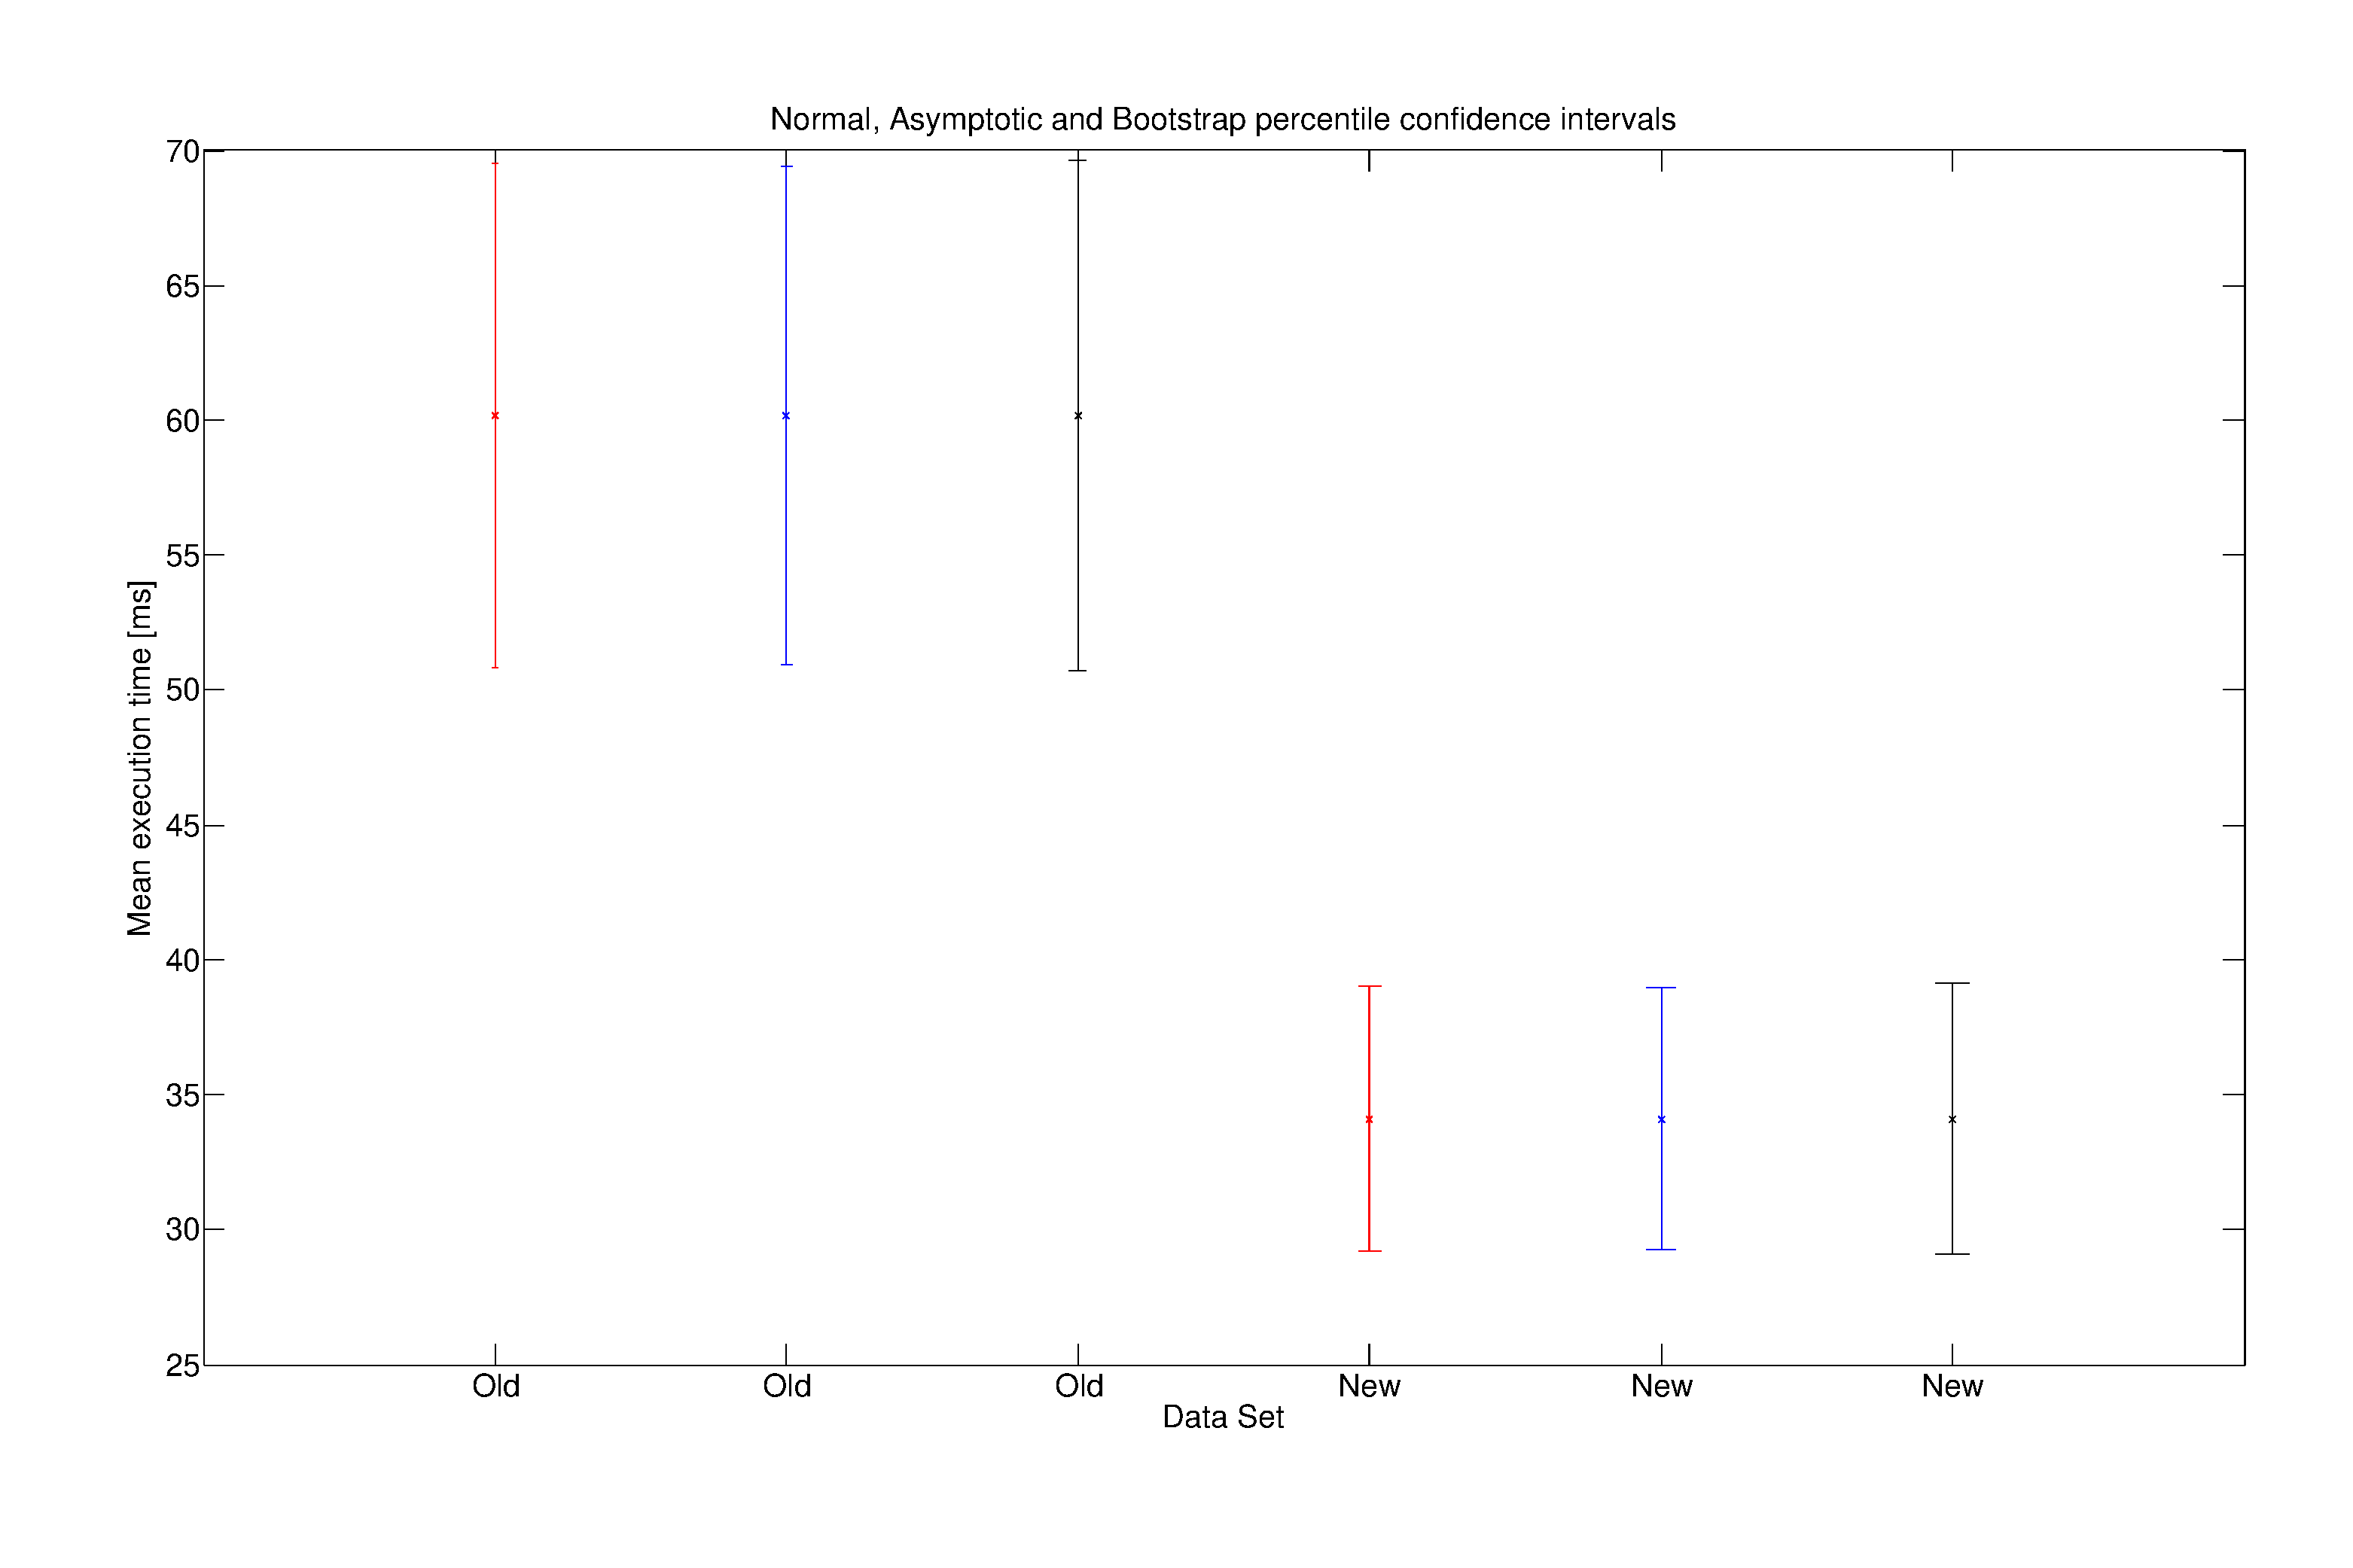
\includegraphics[width=0.7\textwidth]{images/hw1_1_28}
  \caption{Figure 2.8 in \cite{leb}. Different ways to compute confidence intervals for the mean, from left to right, for each dataset: with the assumption that dataset is normal, iid and big dataset, bootstrap method.}
  \label{fig:28}
\end{figure}

\begin{figure}[H]
  \centering
  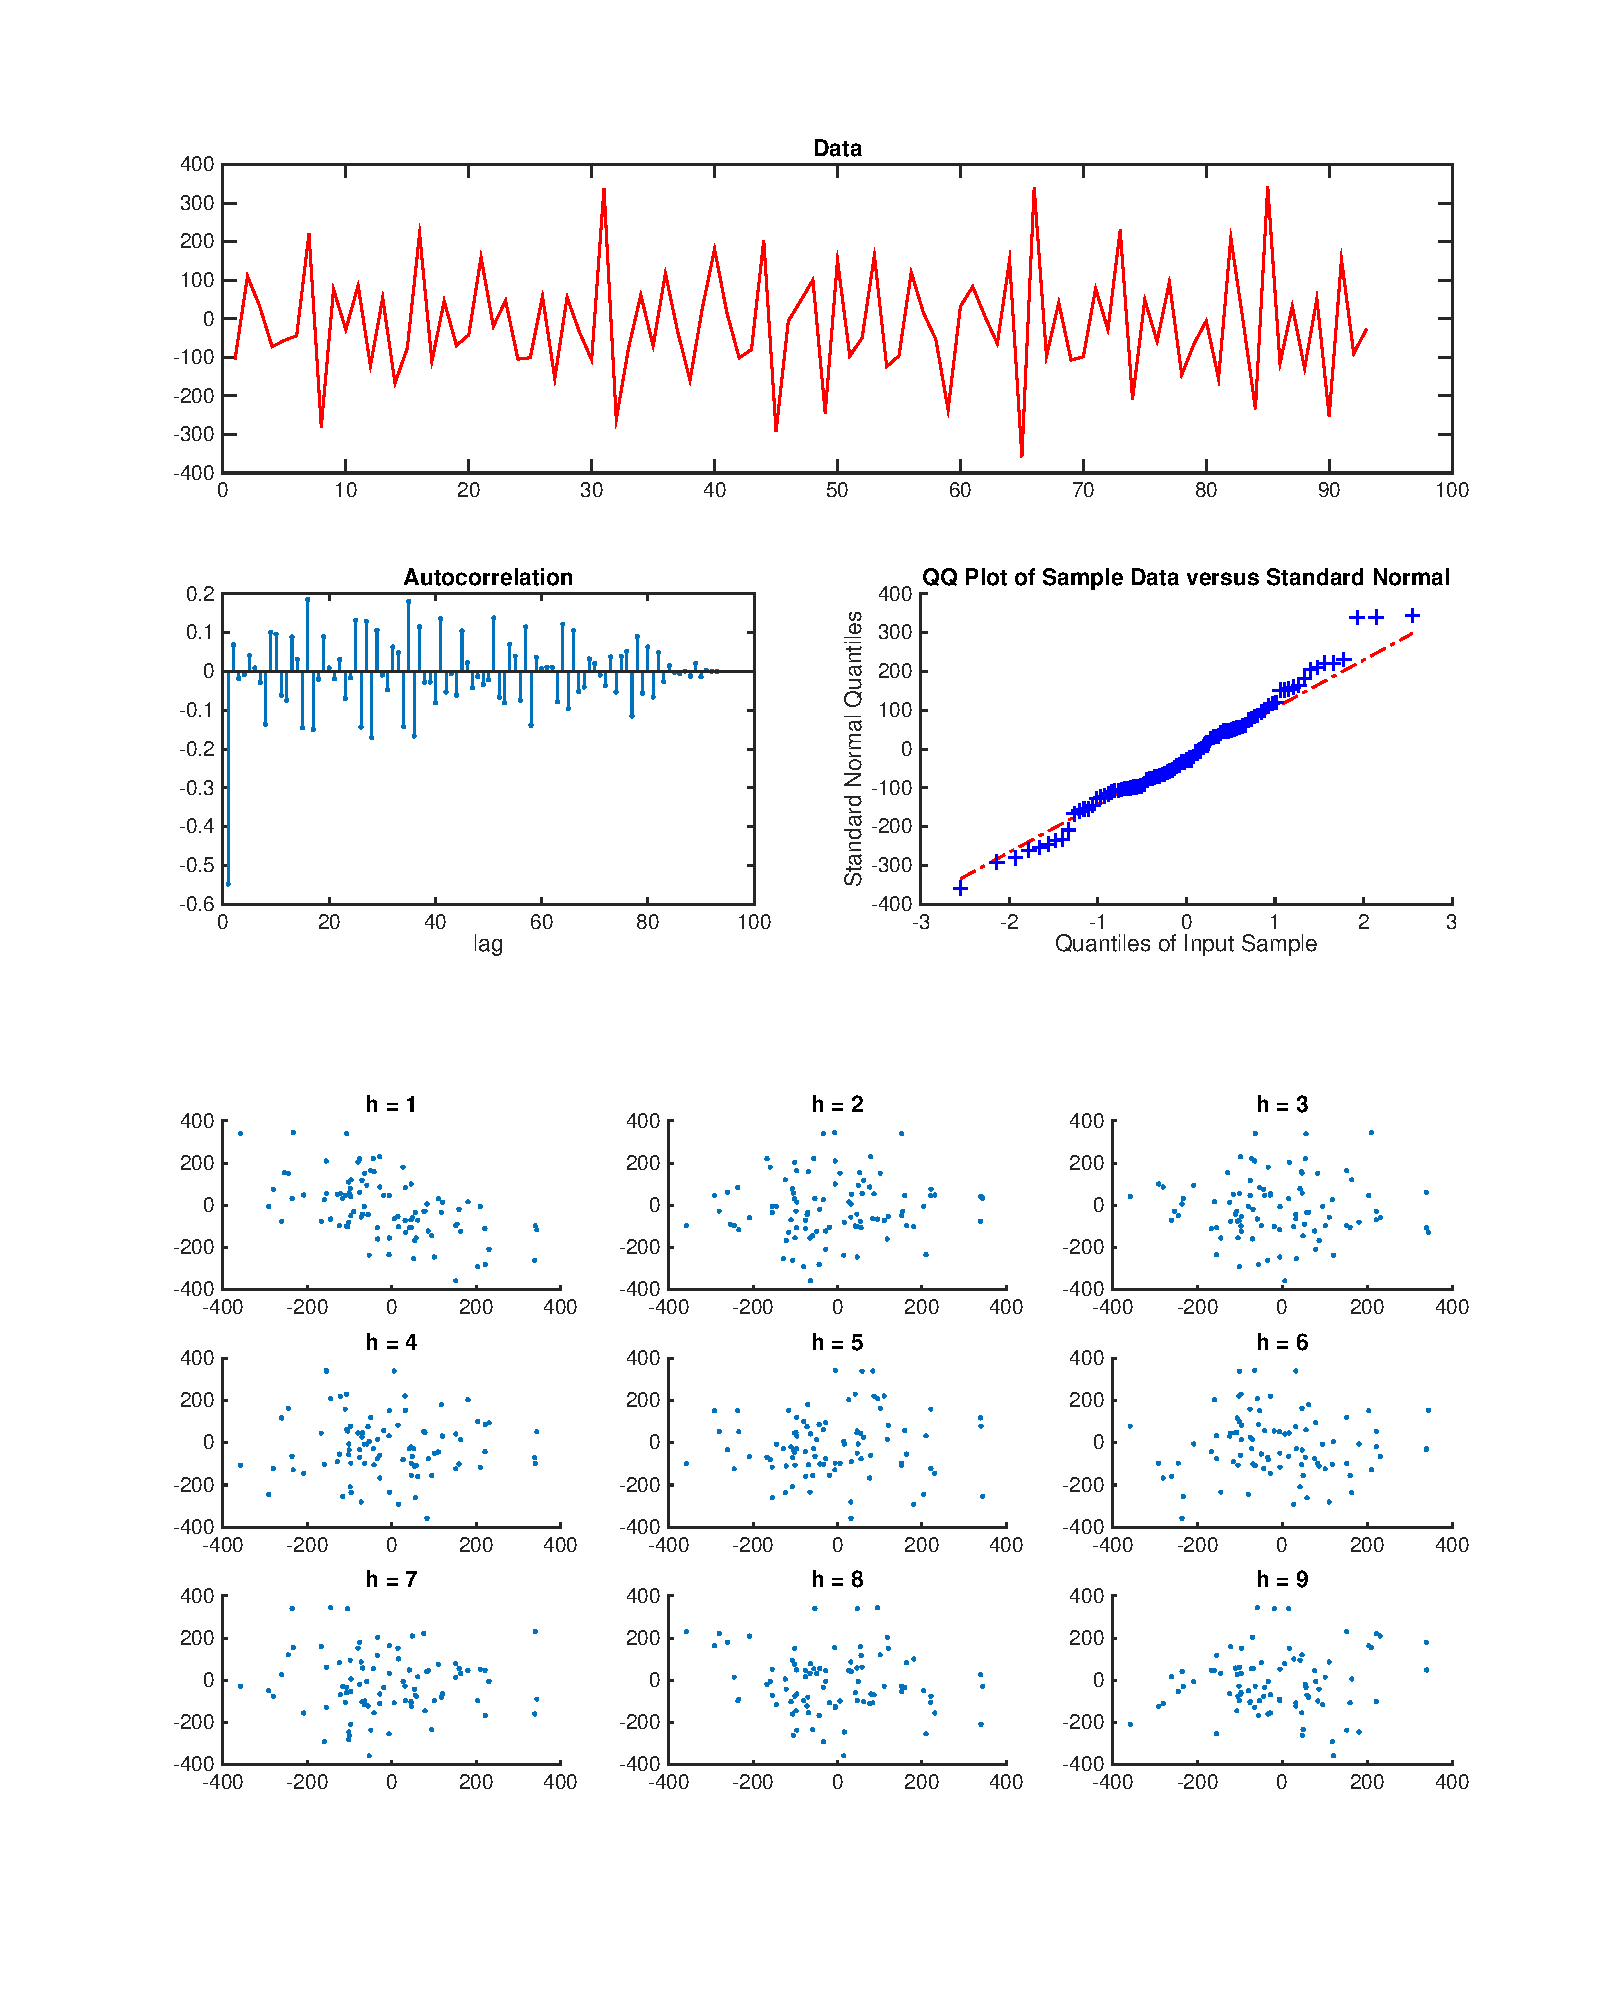
\includegraphics[width=0.8\textwidth, trim=0 80 0 100]{images/hw1_1_210}
  \caption{Figure 2.10 in \cite{leb}. Different ways to visualize iid and normality assumptions.}
  \label{fig:210}
\end{figure}


\FloatBarrier


\section{Exercise 2}
Sample mean and standard deviation are estimated with formulas in Section 1 ($\hat{s}_n = \sqrt{\hat{s}_n^2}$). Confidence interval for the mean of the dataset \{$x_1, ... , x_n$\} is computed as in Theorem 2.2 of \cite{leb}, which can be applied if the dataset is composed of iid samples, the underlying distribution has a finite variance and the number of samples is large. Under these assumptions, given $\hat{\mu}_n$ and $\hat{s}_n$ of the dataset, then the confidence interval is $\hat{\mu}_n \pm \eta \frac{\hat{s}_n}{\sqrt{n}}$ with $\eta$ such that $N_{0,1}(\eta) = \frac{1+\gamma}{2}$. \\
Actually $n=48$ samples are not too many. However the theorem provides a good approximation of the confidence interval for the mean. Let's consider the following experiment: draw for 1000 times, independently, 48 iid  $U[0,1]$ samples at each time and compute the confidence interval at 95\% level as above ($\eta = 1.96$). In Figure~\ref{fig:ci_mean_1000} there's the plot of the 1000 confidence intervals ordered by increasing lower bound. The number of confidence intervals that don't contain the true mean is 49, this means that in $49/1000 \approx 0.05\%$ of the cases the true mean is outside the confidence interval. This respects the definition of confidence interval at 95\% with a little approximation due to the fact that each dataset isn't too big and data is not normal.\\
If instead the experiment is carried out using 48 iid random variables distributed according to a $N[0, 1]$, the confidence interval is given by an exact result from Theorem 2.3 in \cite{leb}. The number of confidence intervals that don't contain the true mean in 1000 trials is 43 (0.043\%), as it can be seen in Figure~\ref{fig:ci_mean_1000_norm}.\\
However if we increase the number of 48-samples dataset generated to $10^6$ then it is possible to see that the percentage of intervals that doesn't contain the true mean grows to expected results, which are 5.378\% for U[0,1] (it is still an approximation with few non normal samples) and 4.9978\% for N[0,1] ($\approx 5\%$ according to the definition).\\

\begin{figure}[h!]
  \centering
  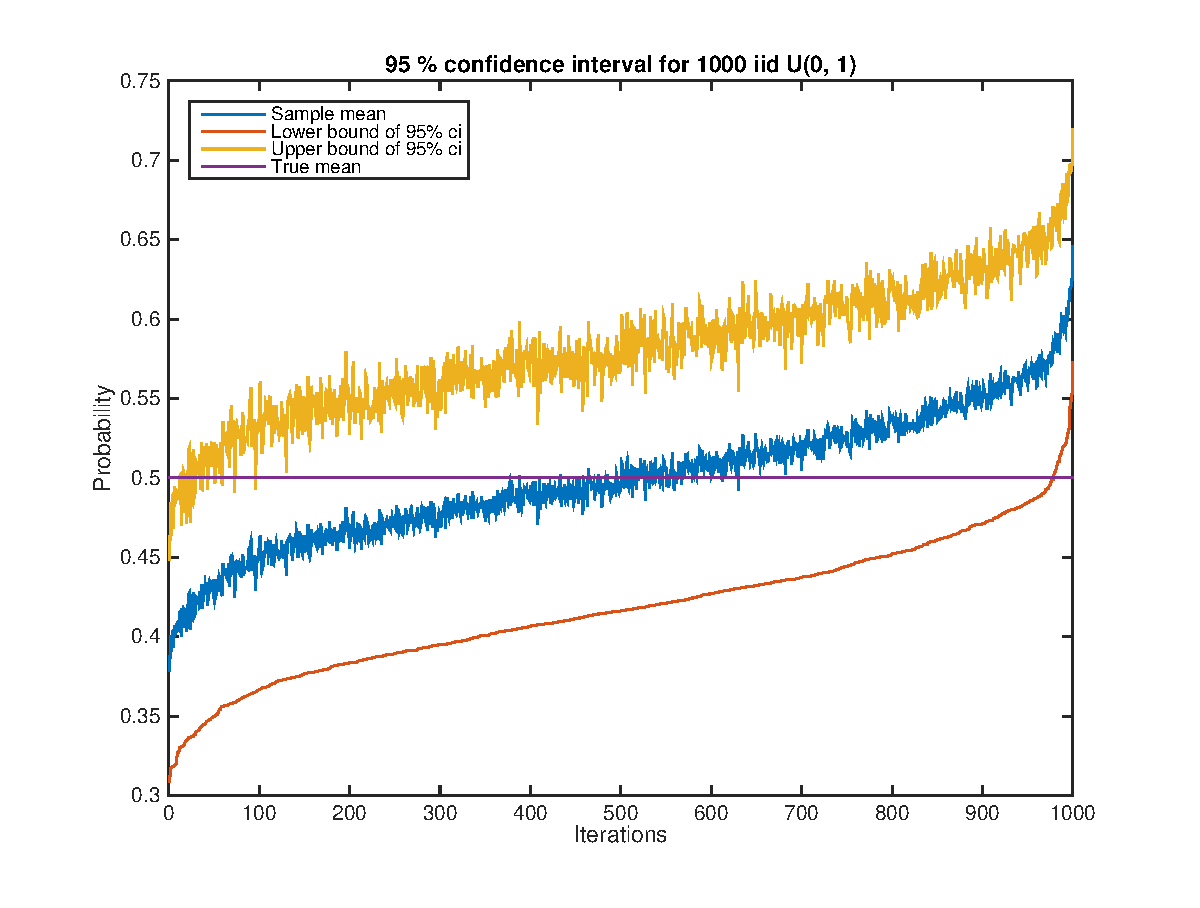
\includegraphics[width = 0.7\textwidth]{images/hw1_2_c_uni}
  \caption{1000 confidence intervals, each computed for 48 iid rv U[0,1]}
  \label{fig:ci_mean_1000}
\end{figure}

\clearpage

\begin{figure}[htp]
  \centering
  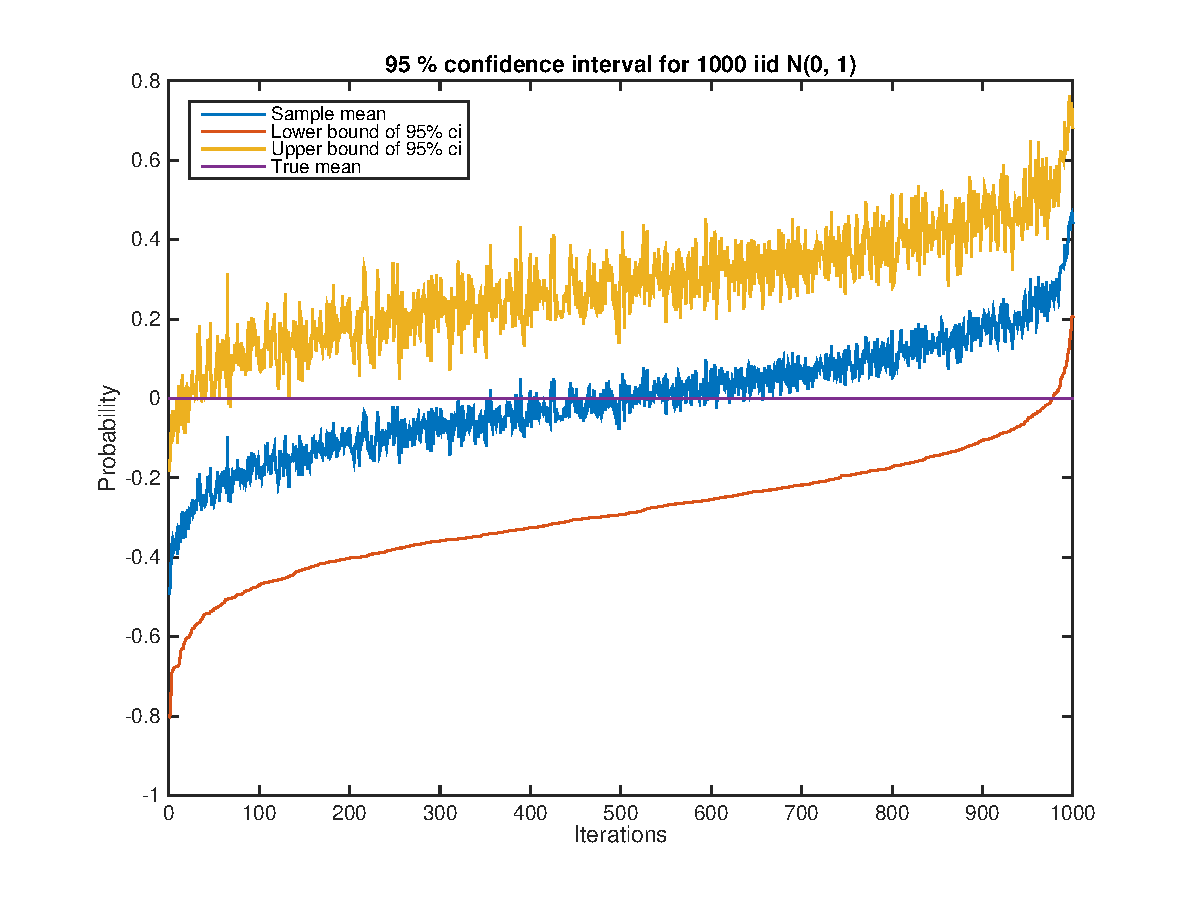
\includegraphics[width = 0.7\textwidth]{images/hw1_2_c}
  \caption{1000 confidence intervals, each computed for 48 iid rv N[0,1]}
  \label{fig:ci_mean_1000_norm}
\end{figure}


\section{Exercise 3}
Consider a dataset $\{X_1, ..., X_n\}$ and its order statistic $X_{(1)}^n, ..., X_{(n)}^n$. $X_{(1)}^n$ is the lowest value in $\{X_1, ..., X_n\}$, $X_{(i)}^n$ is the $i-th$ lowest value in $\{X_1, ..., X_n\}$ and so on. If the $i-th$ element in the order statistic is equal to $y$, then there are $i-1$ samples lower or equal than $y$ (each with probability $P[X\le y] = F_X(y)$) and $n-i$ samples greater than $y$ (each with probability $P[X > y] = 1 - F_X(y)$). This can be described with a multinomial distribution (see \cite{pk}):
\begin{multline}
P[X_{(i)}^n = y] = f_{X_{(i)}^n}(y) = \frac{n!}{(i-1)!1!(n-i)!}(P[X\le y]^{(i-1)}) P[X = y] (P[X > y]^{(n-i)}) = \\ = \frac{n!}{(i-1)!(n-i)!} F_X(y)^{(i-1)} f_X(y) [1-F_X(y)]^{(n-i)}
\label{eq:pdf_gen}
\end{multline}
where the first term is a coefficient of the multinomial distribution, the second is the probability that $i - 1$ samples are lower or equal than $y$, the third is the density of the i-th sample itself, and eventually the fourth is the probability that $n - i$ samples are greater than $y$. \\
If $X$ is $U[0,1]$ then $f_X(y) = 1$ and $F_X(y) = y$ with $y \in [0,1]$ so Equation~\ref{eq:pdf_gen} becomes
\begin{equation}
  f_{X_{(i)}^n}(y) = \frac{n!}{(i-1)!(n-i)!} y^{i-1} (1-y)^{n-i}
\end{equation}
which is a beta distribution with $\alpha = i$ and $\beta = n - i + 1$. So $E[X_{(i)}^n]= \frac{i}{n+1}$ as reported in \cite{pk}.


\section{Exercise 4}
This experiment is designed in order to study how does the accuracy of estimates of mean and variance improve by increasing the size of the dataset on which they are computed, both in the $U[0,1]$ and $N[0,1]$ cases. For the sample mean of a dataset \{$x_1, ... , x_n$\} the variance of the estimator is $\frac{\hat{s}^2_n}{\sqrt{n}}$ so we should expect that the accuracy increases as $n$ gets bigger. \\
This behavior can be observed in Figures~\ref{fig:uni_n} and~\ref{fig:norm_n}, with the plot of sample mean and sample variance as functions of the dataset size $n$, computed with estimators of Section 1. For small $n$ the estimate is bad, while it tends to the true value of the mean and standard deviation for higher values of $n$. \\

\begin{figure}[h]
  \centering
  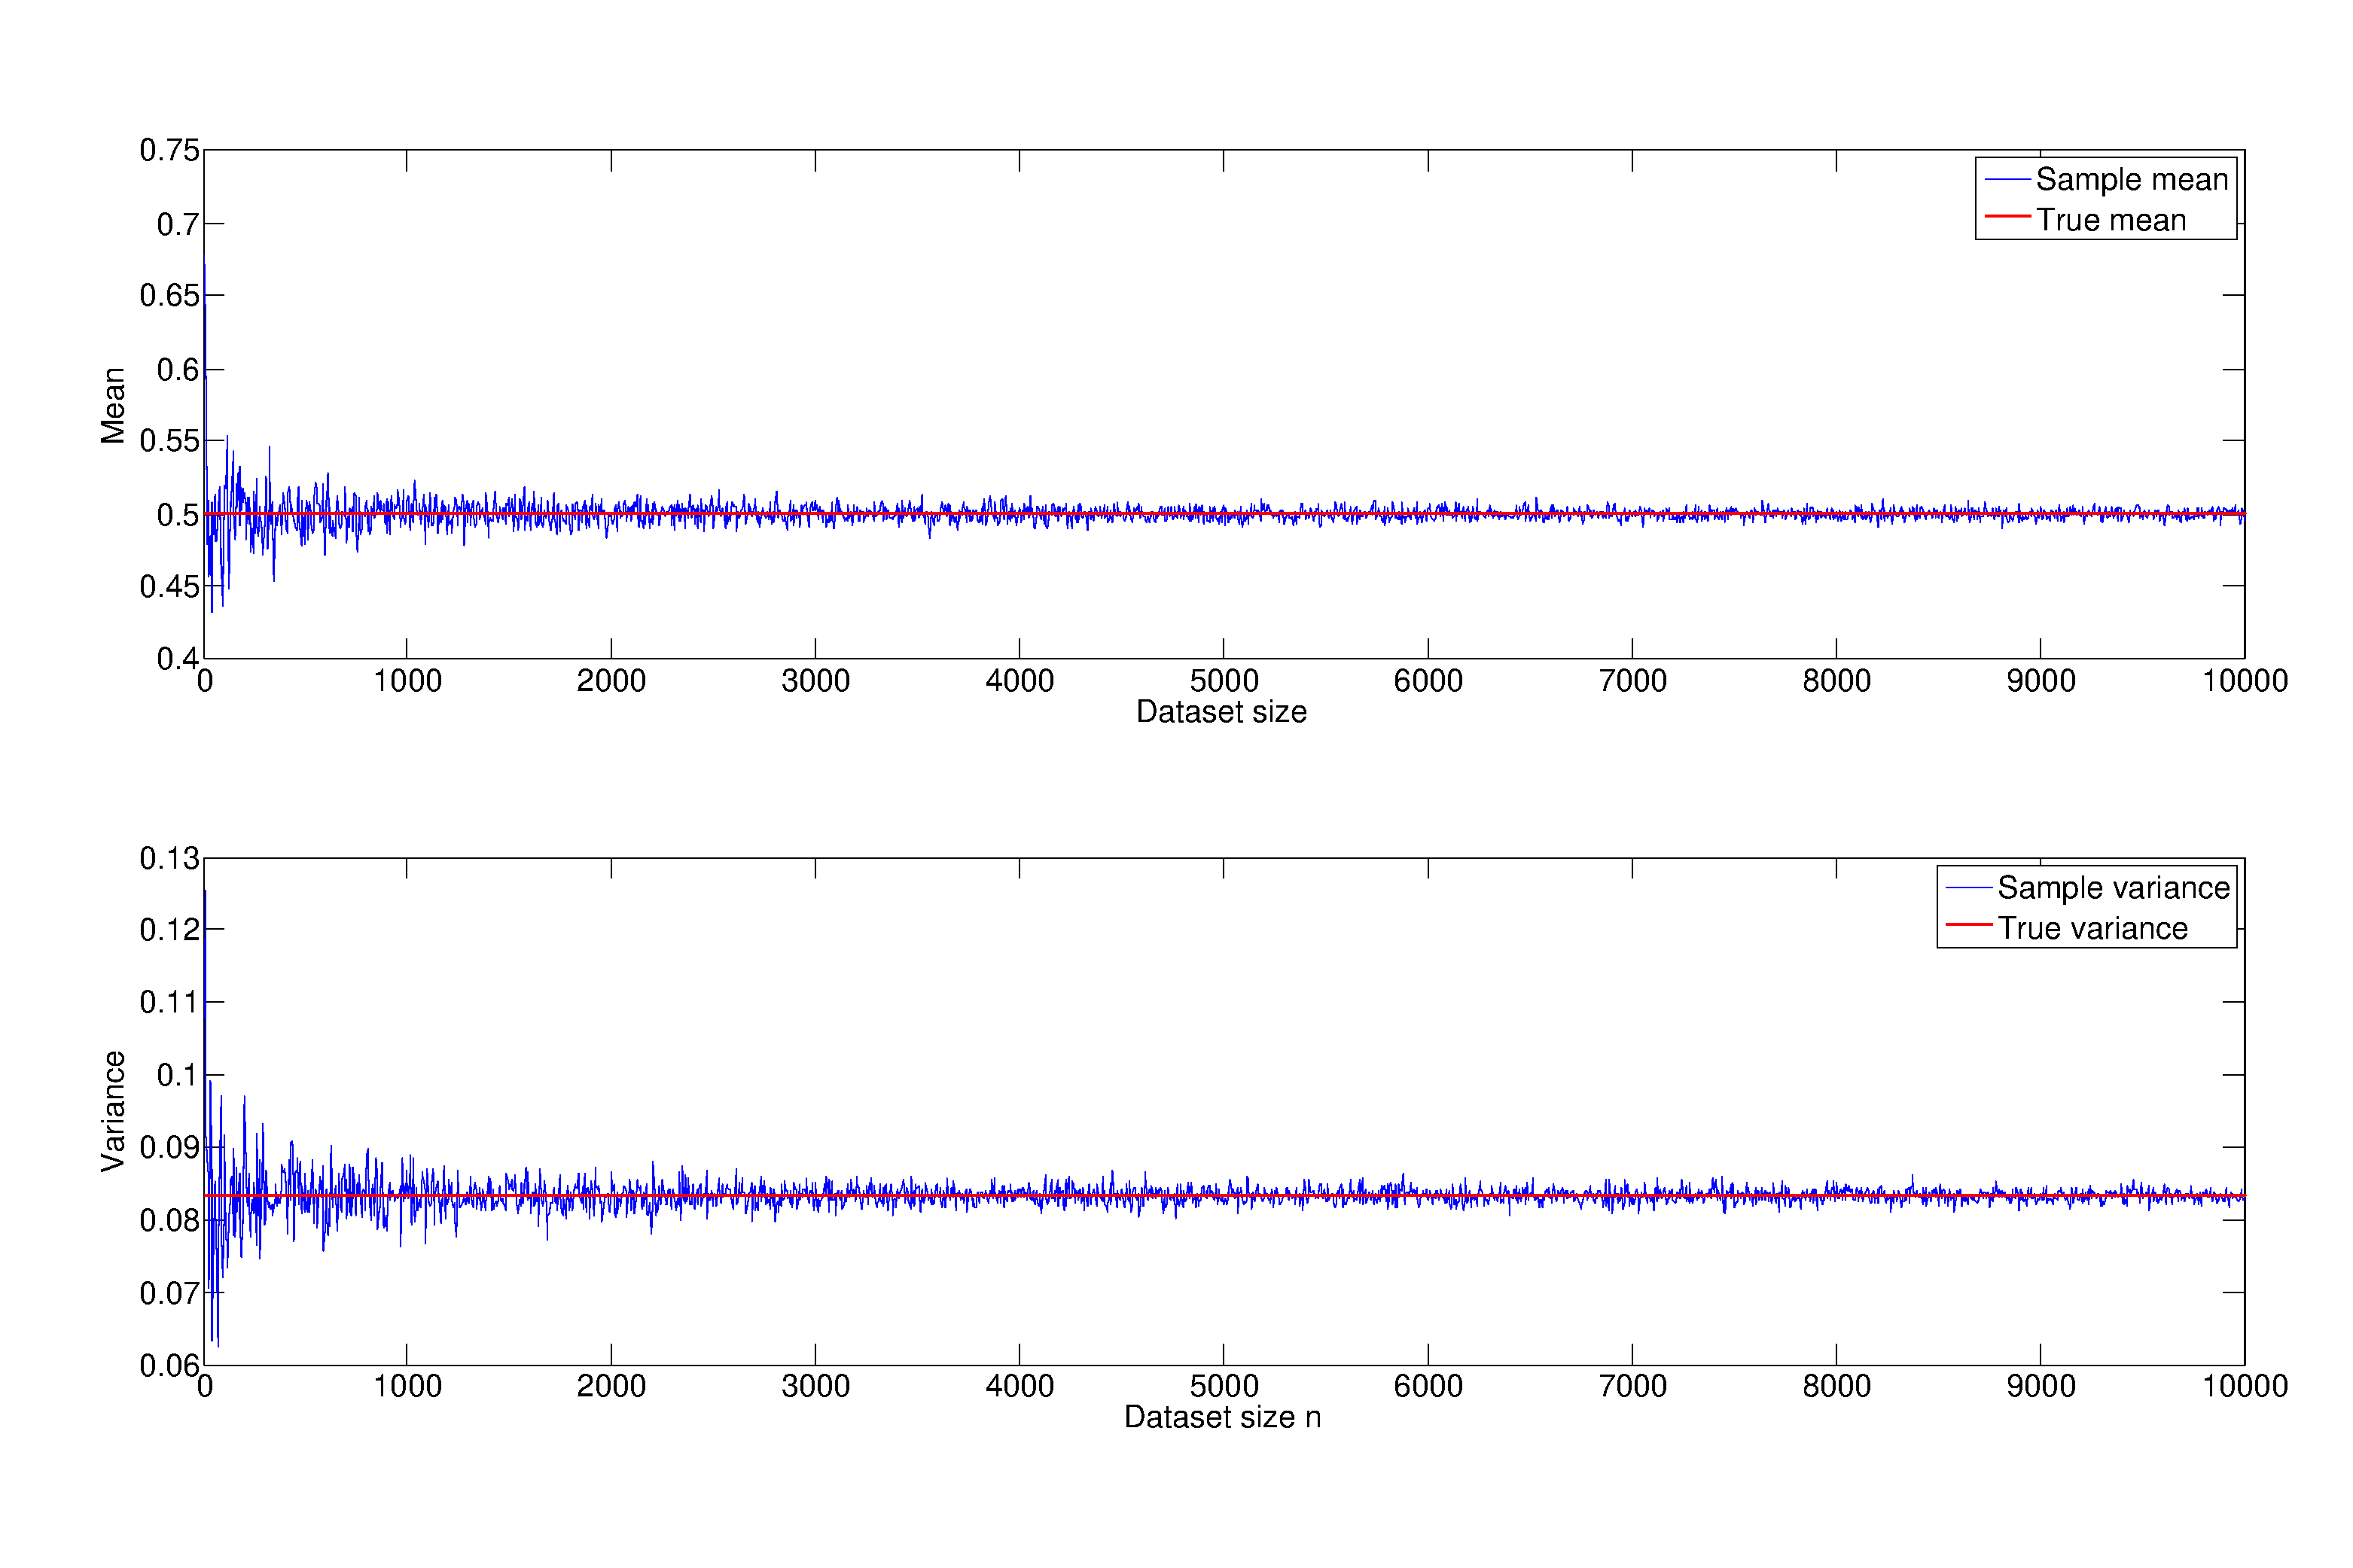
\includegraphics[width=0.7\textwidth]{images/hw1_4_a_uni}
  \caption{Sample mean and sample variance for $U[0,1]$ as a function of dataset size $n$}
  \label{fig:uni_n}
\end{figure}


\begin{figure}[h]
  \centering
  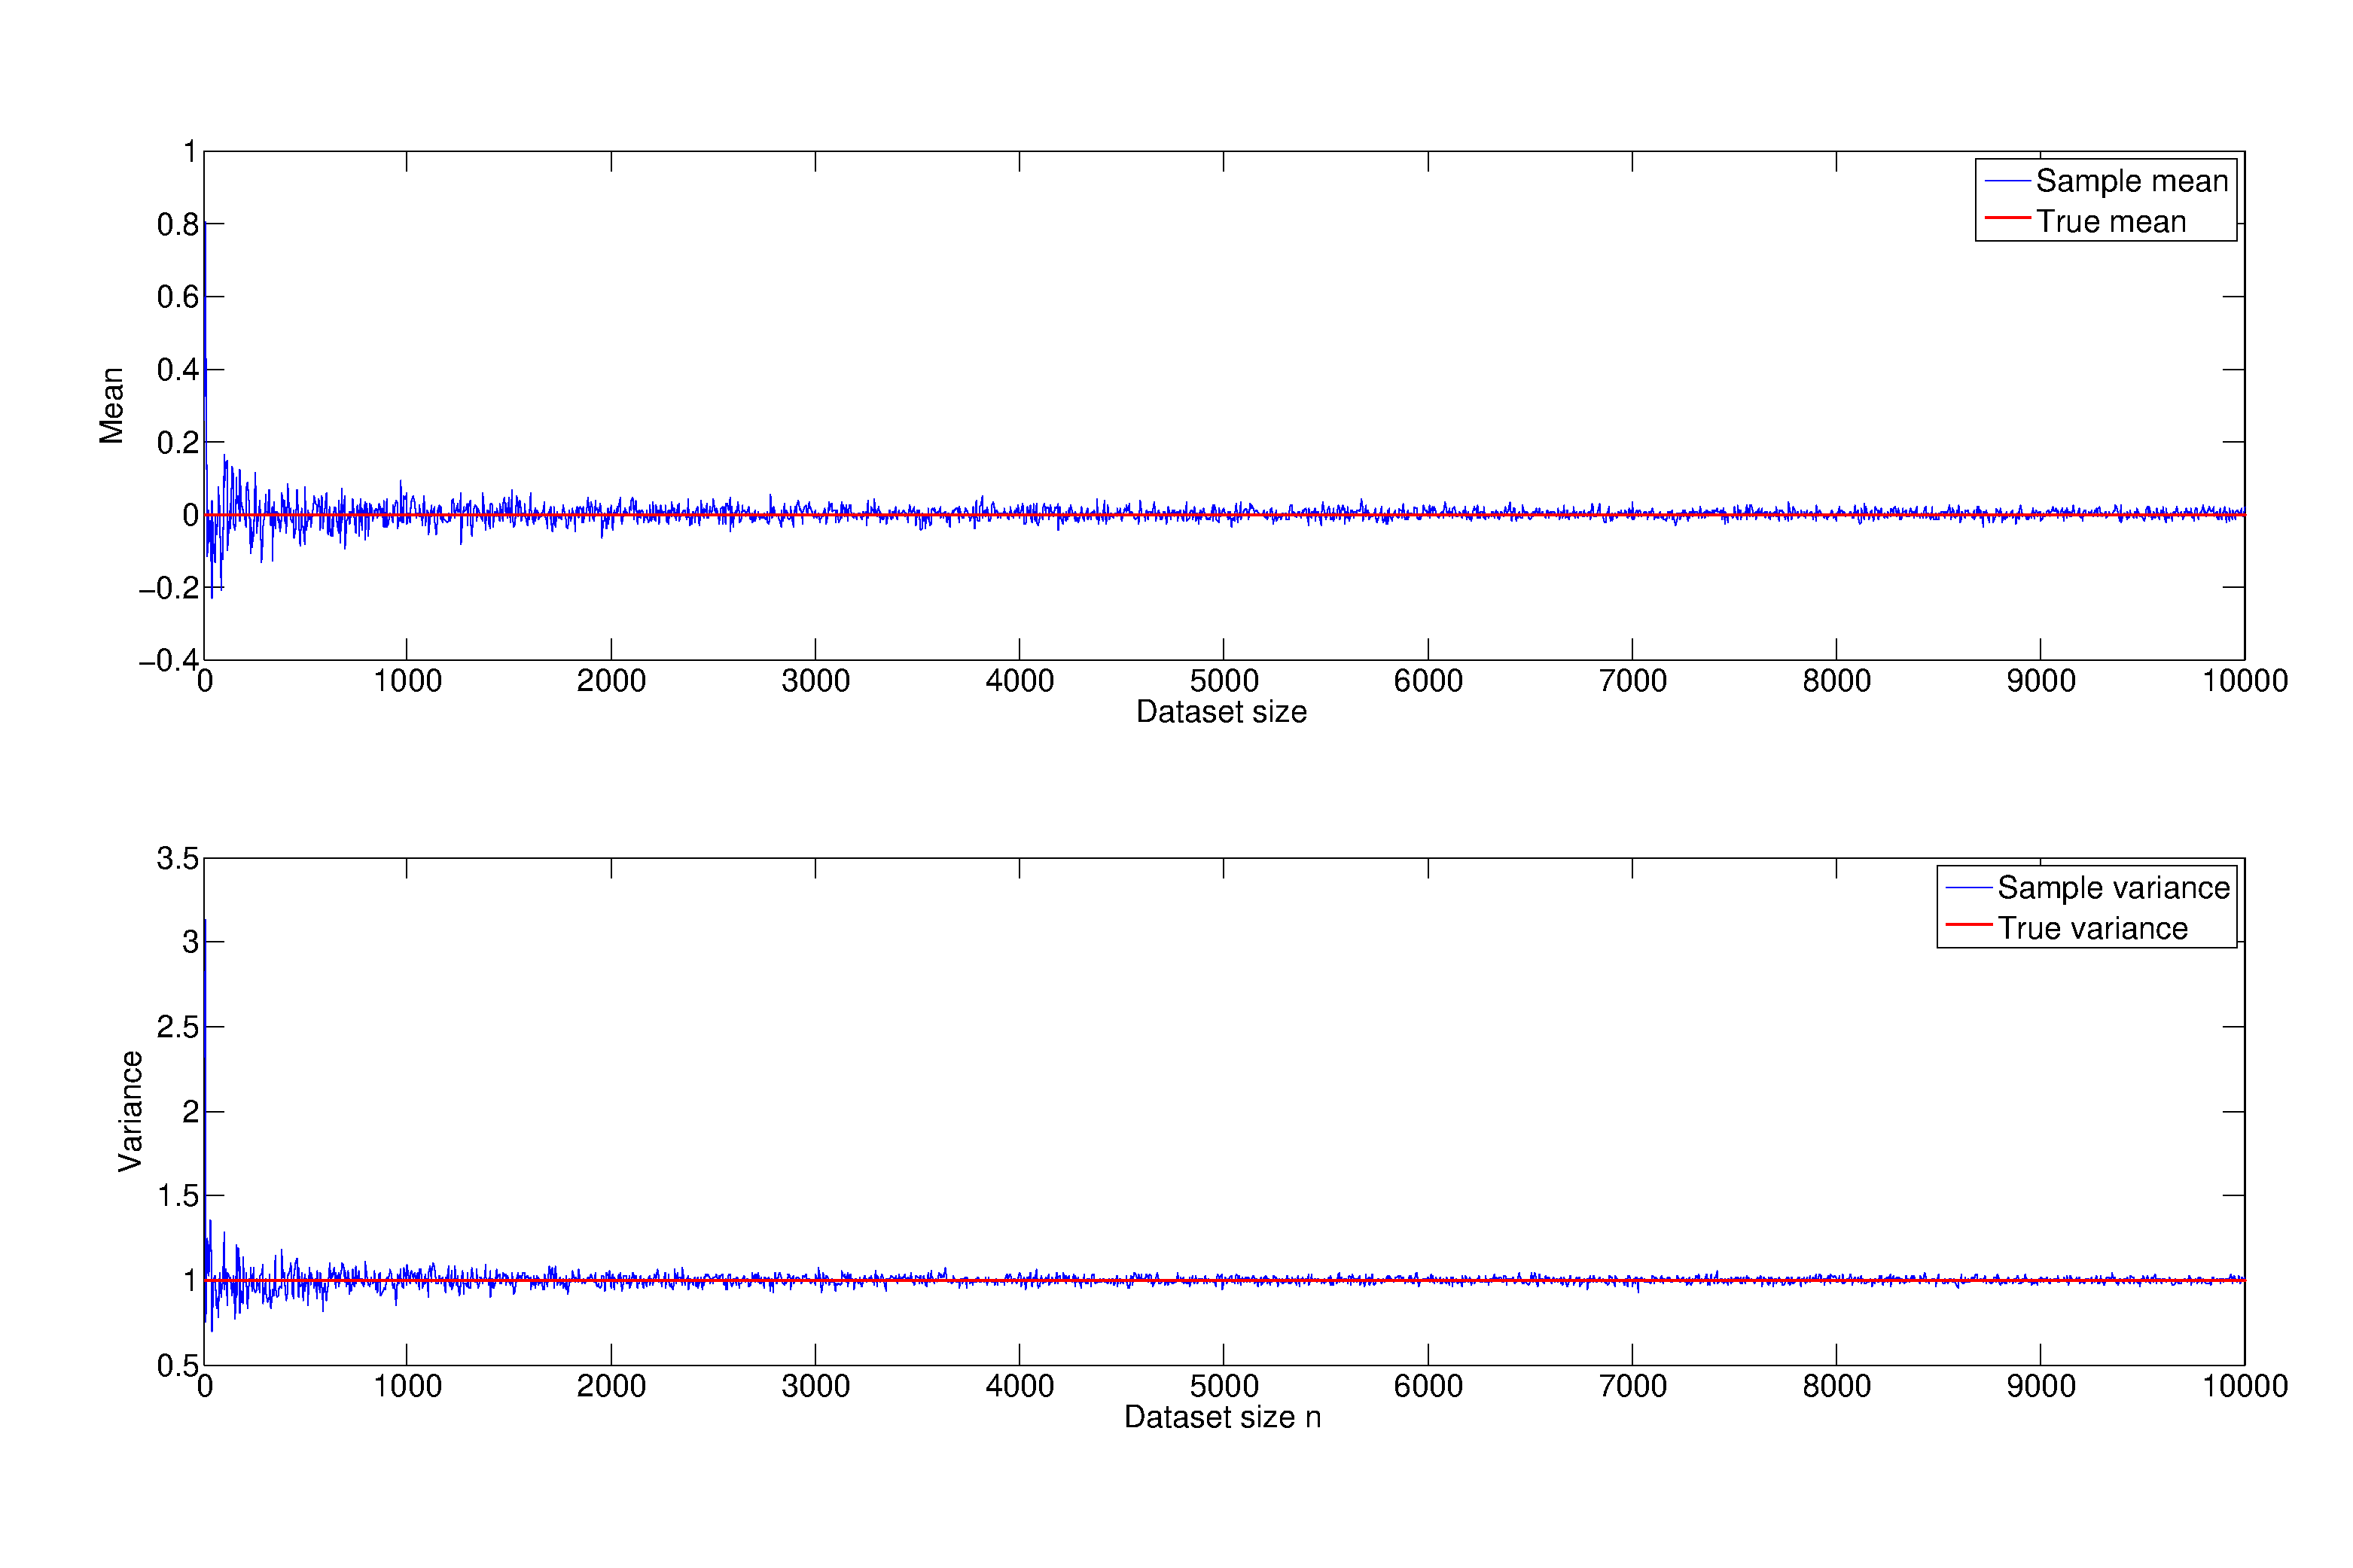
\includegraphics[width=0.7\textwidth]{images/hw1_4_a_norm}
  \caption{Sample mean and sample variance for $N[0,1]$ as a function of dataset size $n$}
  \label{fig:norm_n}
\end{figure}

\subsubsection*{Confidence Intervals for variance}

If dataset isn't normal there is not a theoretical result that can be used to exactly compute confidence intervals for variance. The only way is to use the bootstrap method, which involves a simulation and the usage of 2 percentiles as confidence intervals, as it can be seen in the following code.
\lstinputlisting{../code/bootstrap_var.m}
The extraction with replacement of the samples from the dataset could be performed using a uniform random variable in the interval $[0, n]$ with $n$ the size of the dataset, however MATLAB provides function \verb datasample  with the same functionality.\\
The confidence interval at 95\% level gets closer to the value of the true variance as $n$ increases as it can be seen in~\ref{fig:uni_n_var}, this means that the estimate is more accurate in the 95\% of the cases in which the true variance is included in the confidence interval. \\
\begin{figure}[h!]
  \centering
  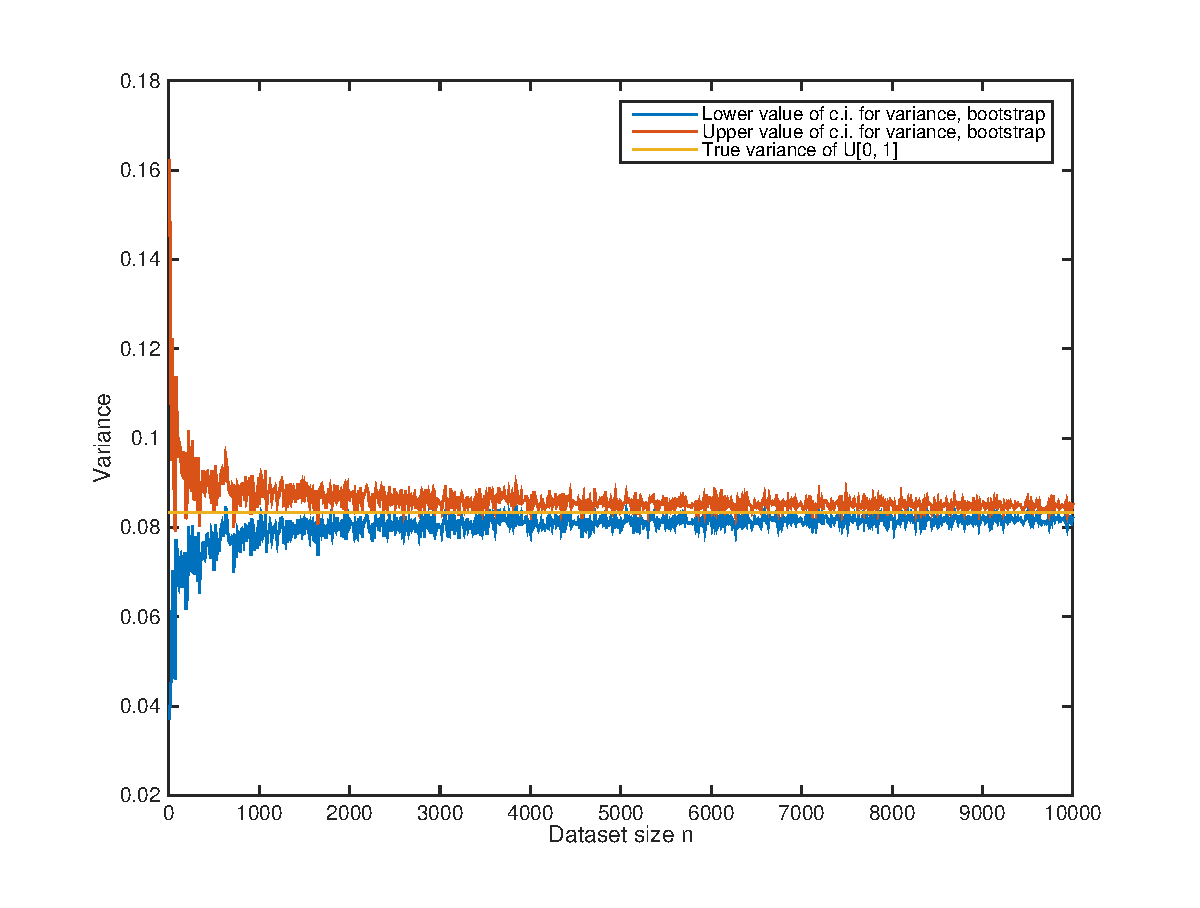
\includegraphics[width=0.6\textwidth]{images/hw1_4_c_uni}
  \caption{Confidence intervals for the variance of $U[0,1]$ as a function of dataset size $n$}
  \label{fig:uni_n_var}
\end{figure}

If the data is normal, instead, the distribution of $(n-1)\frac{\hat{s}_n^2}{\sigma^2}$ is $\chi_{n-1}^2$ and confidence interval for level $\gamma$ can be computed exactly as $\big[\hat{s}_n\sqrt{\frac{n-1}{\xi}}, \hat{s}_n\sqrt{\frac{n-1}{\zeta}}\big]$ with $\xi$, $\zeta$ such that $\chi_{n-1}^2 (\xi) = \frac{1 -\gamma}{2}$ and $\chi_{n-1}^2 (\zeta) = \frac{1 +\gamma}{2}$. \\
The bootstrapped and theoretically computed confidence intervals for a $N[0,1]$ are in Figures~\ref{fig:norm_n_var} and~\ref{fig:norm_n_var_chi}.


\begin{figure}[htp]
  \centering
  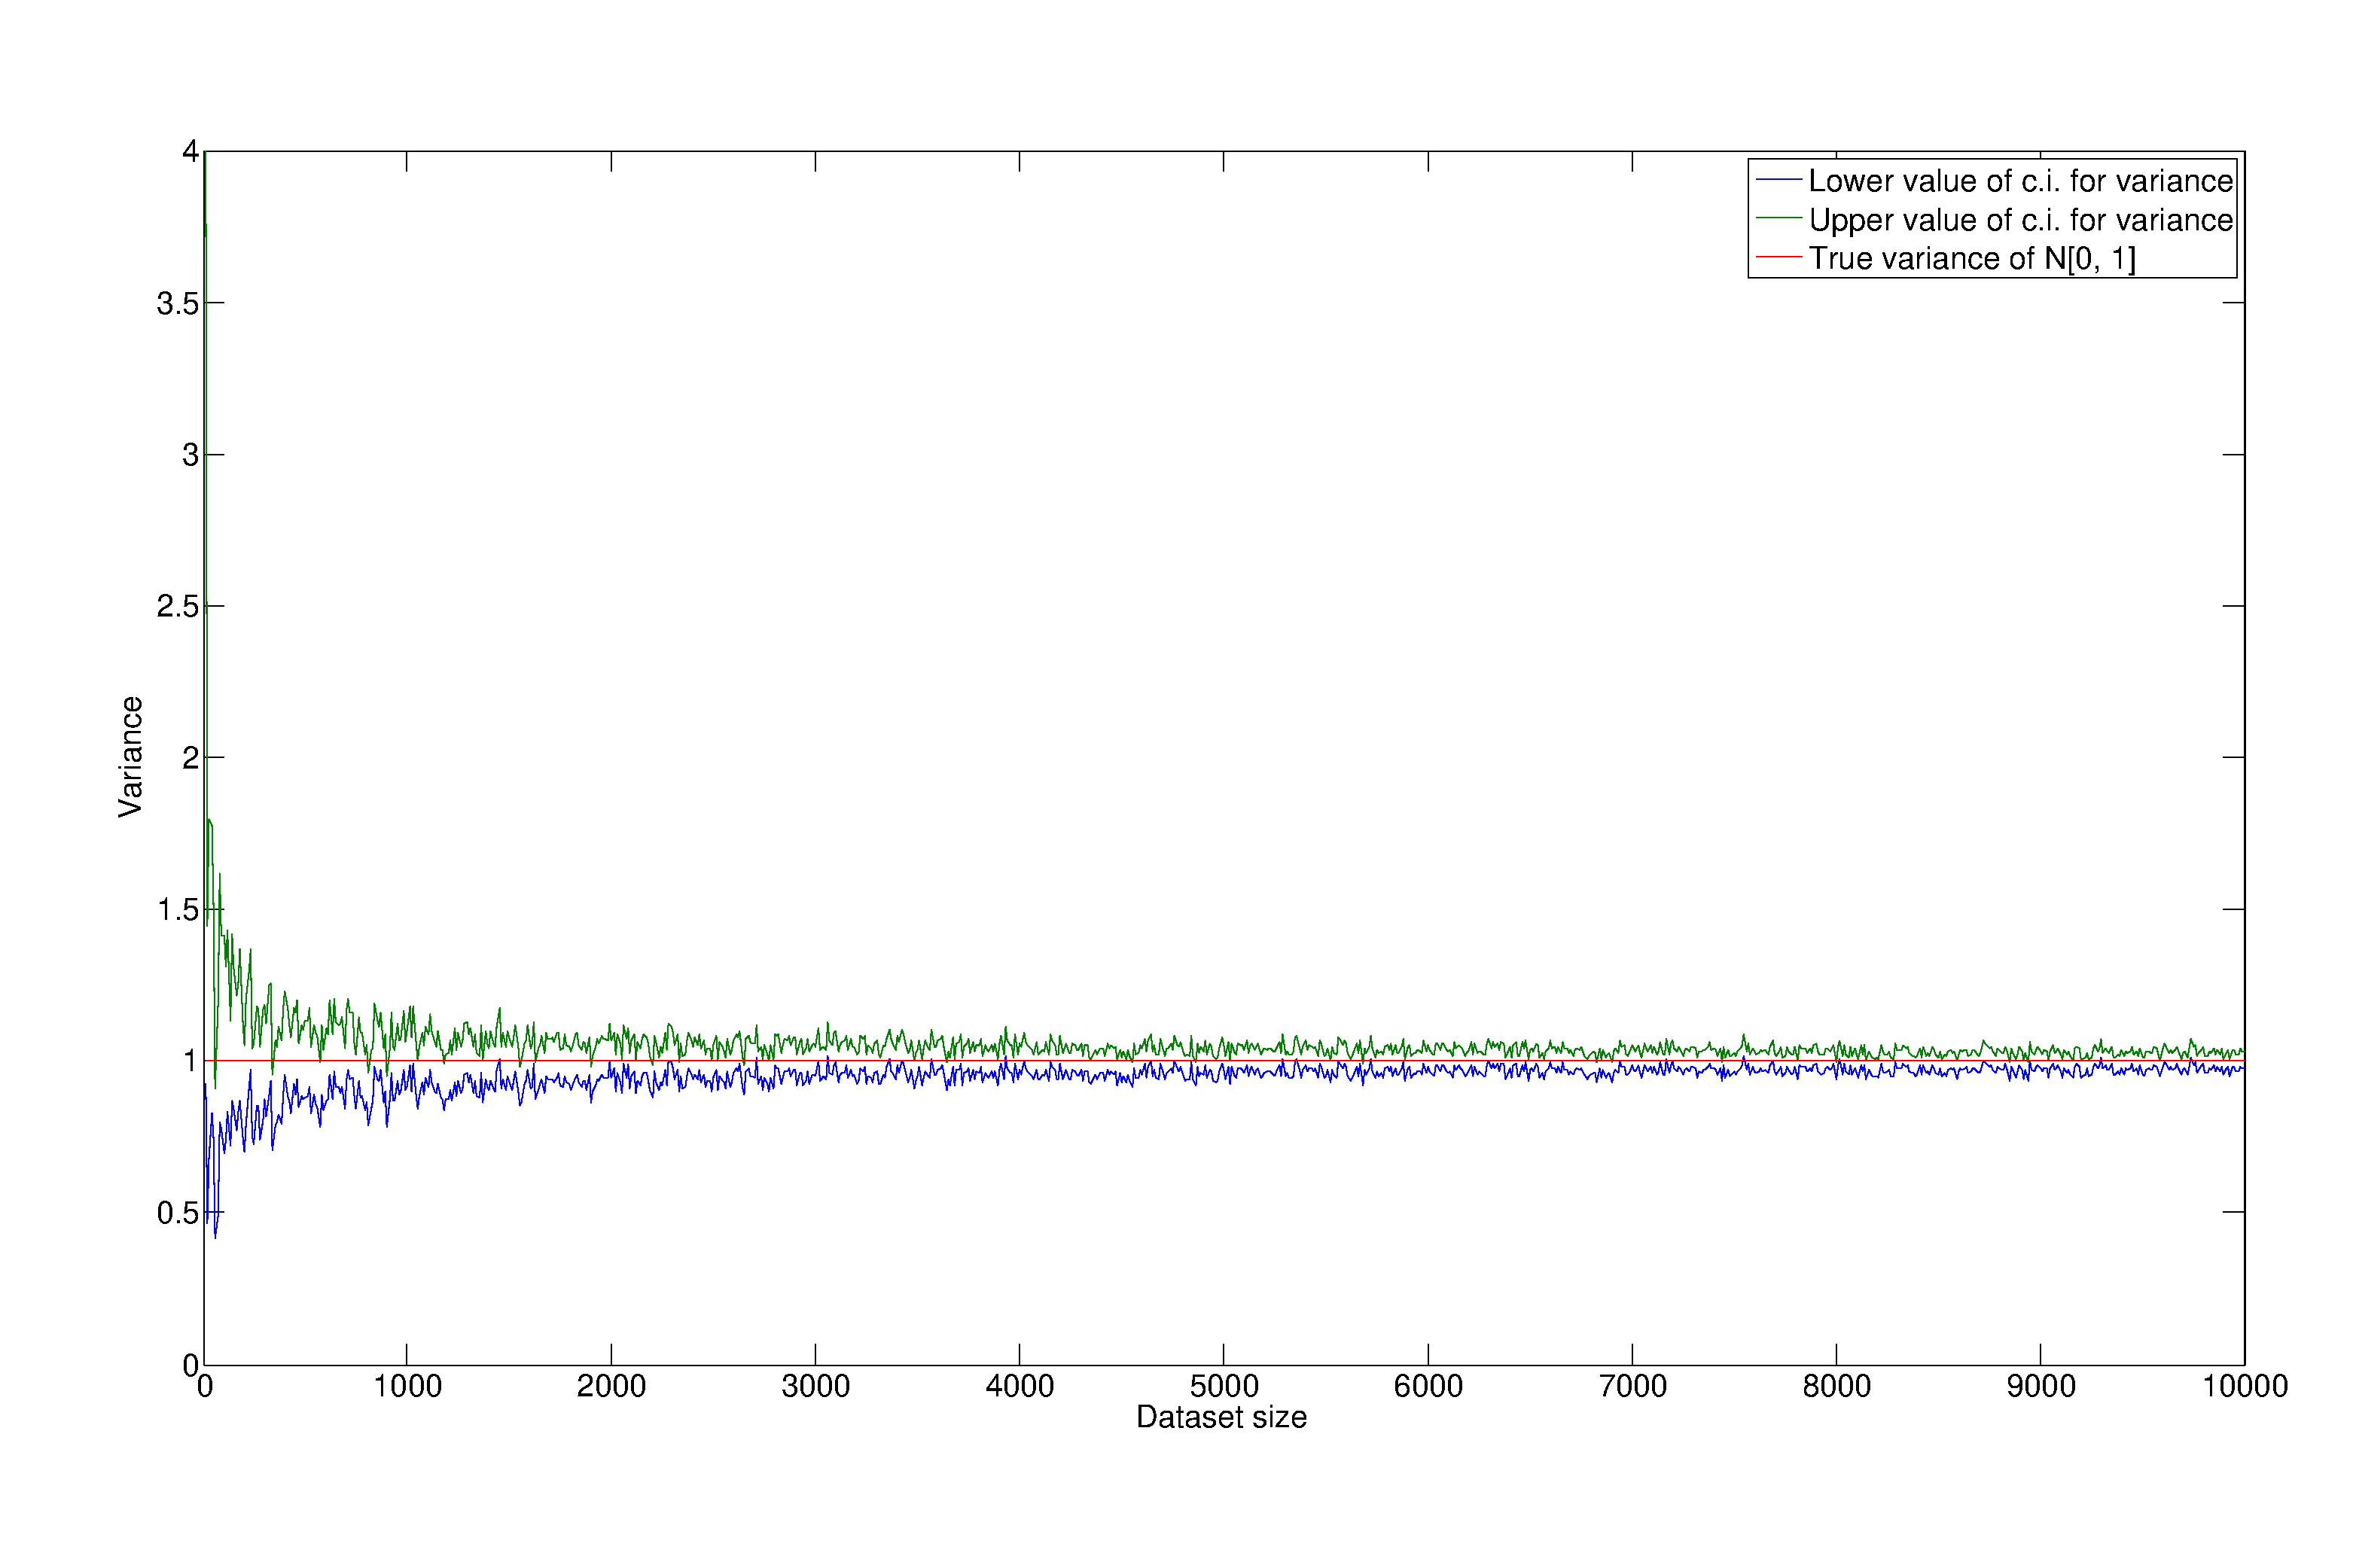
\includegraphics[width=0.6\textwidth]{images/hw1_4_c_norm}
  \caption{Bootstrapped confidence intervals for the variance of $N[0,1]$ as a function of dataset size $n$}
  \label{fig:norm_n_var}
\end{figure}

\begin{figure}[h]
  \centering
  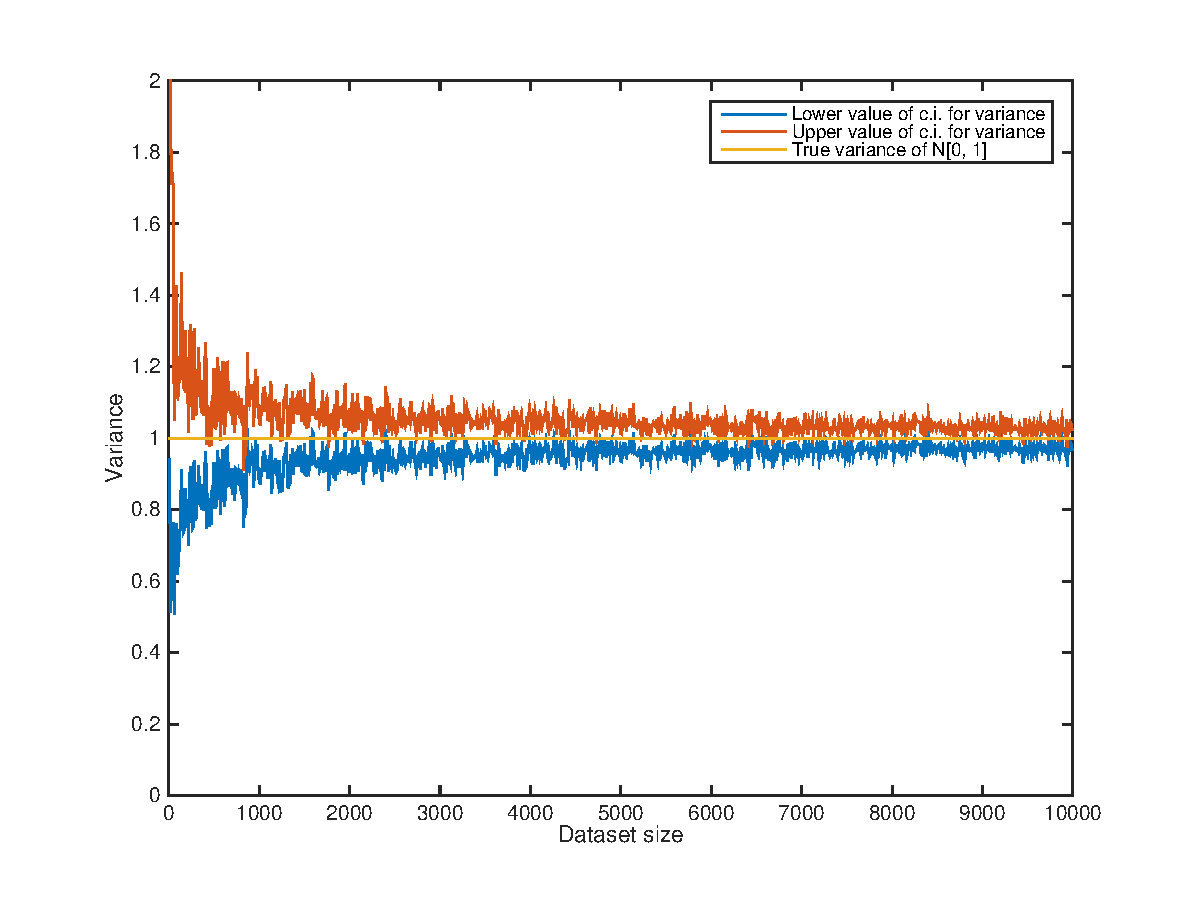
\includegraphics[width=0.6\textwidth]{images/hw1_4_c_norm_chi}
  \caption{Theoretically computed confidence intervals for the variance of $N[0,1]$ as a function of dataset size $n$}
  \label{fig:norm_n_var_chi}
\end{figure}

\FloatBarrier

\subsubsection*{Prediction Intervals}
While a confidence interval describes the accuracy of an estimator, a prediction interval is the interval in which with a certain level of confidence $\gamma$ the sample $X_{n+1}$ of the sequence \{$X_1, ... , X_{n+1}$\} can be found, given that $X_1, ..., X_n$ are known and $X_{n+1}$ hasn't been observed yet. \\
For iid datasets there's a result which is based on order statistic, similar to the bootstrap, but exact. In particular Theorem 2.5 in \cite{leb} states that given the order statistic $X_{(1)}^n, ..., X_{(n)}^n$, for $1 \le j \le k \le n$, $P(X_{(j)}^n \le X_{n+1} \le X_{(k)}^n) = \frac{k-j}{n+1}$. For $1 - \gamma = \alpha \ge \frac{2}{n+1}$ then the prediction interval is $[X_{(j)}, X_{(k)}]$ with $j = \floor{(n+1)\frac{\alpha}{2}}$ and $k = \ceil{(n+1)(1-\frac{\alpha}{2})}$.

Figure~\ref{fig:alpha} plots $\alpha = 0.05$ (for a 95\% prediction level) against $\frac{2}{n+1}$ and it can be seen that for $n \ge 39$ it is possible to compute exactly the prediction interval, which can be found in Figure~\ref{fig:pi_uni}. It is compared with the dataset size $n$.


\begin{figure}[h!]
  \centering
  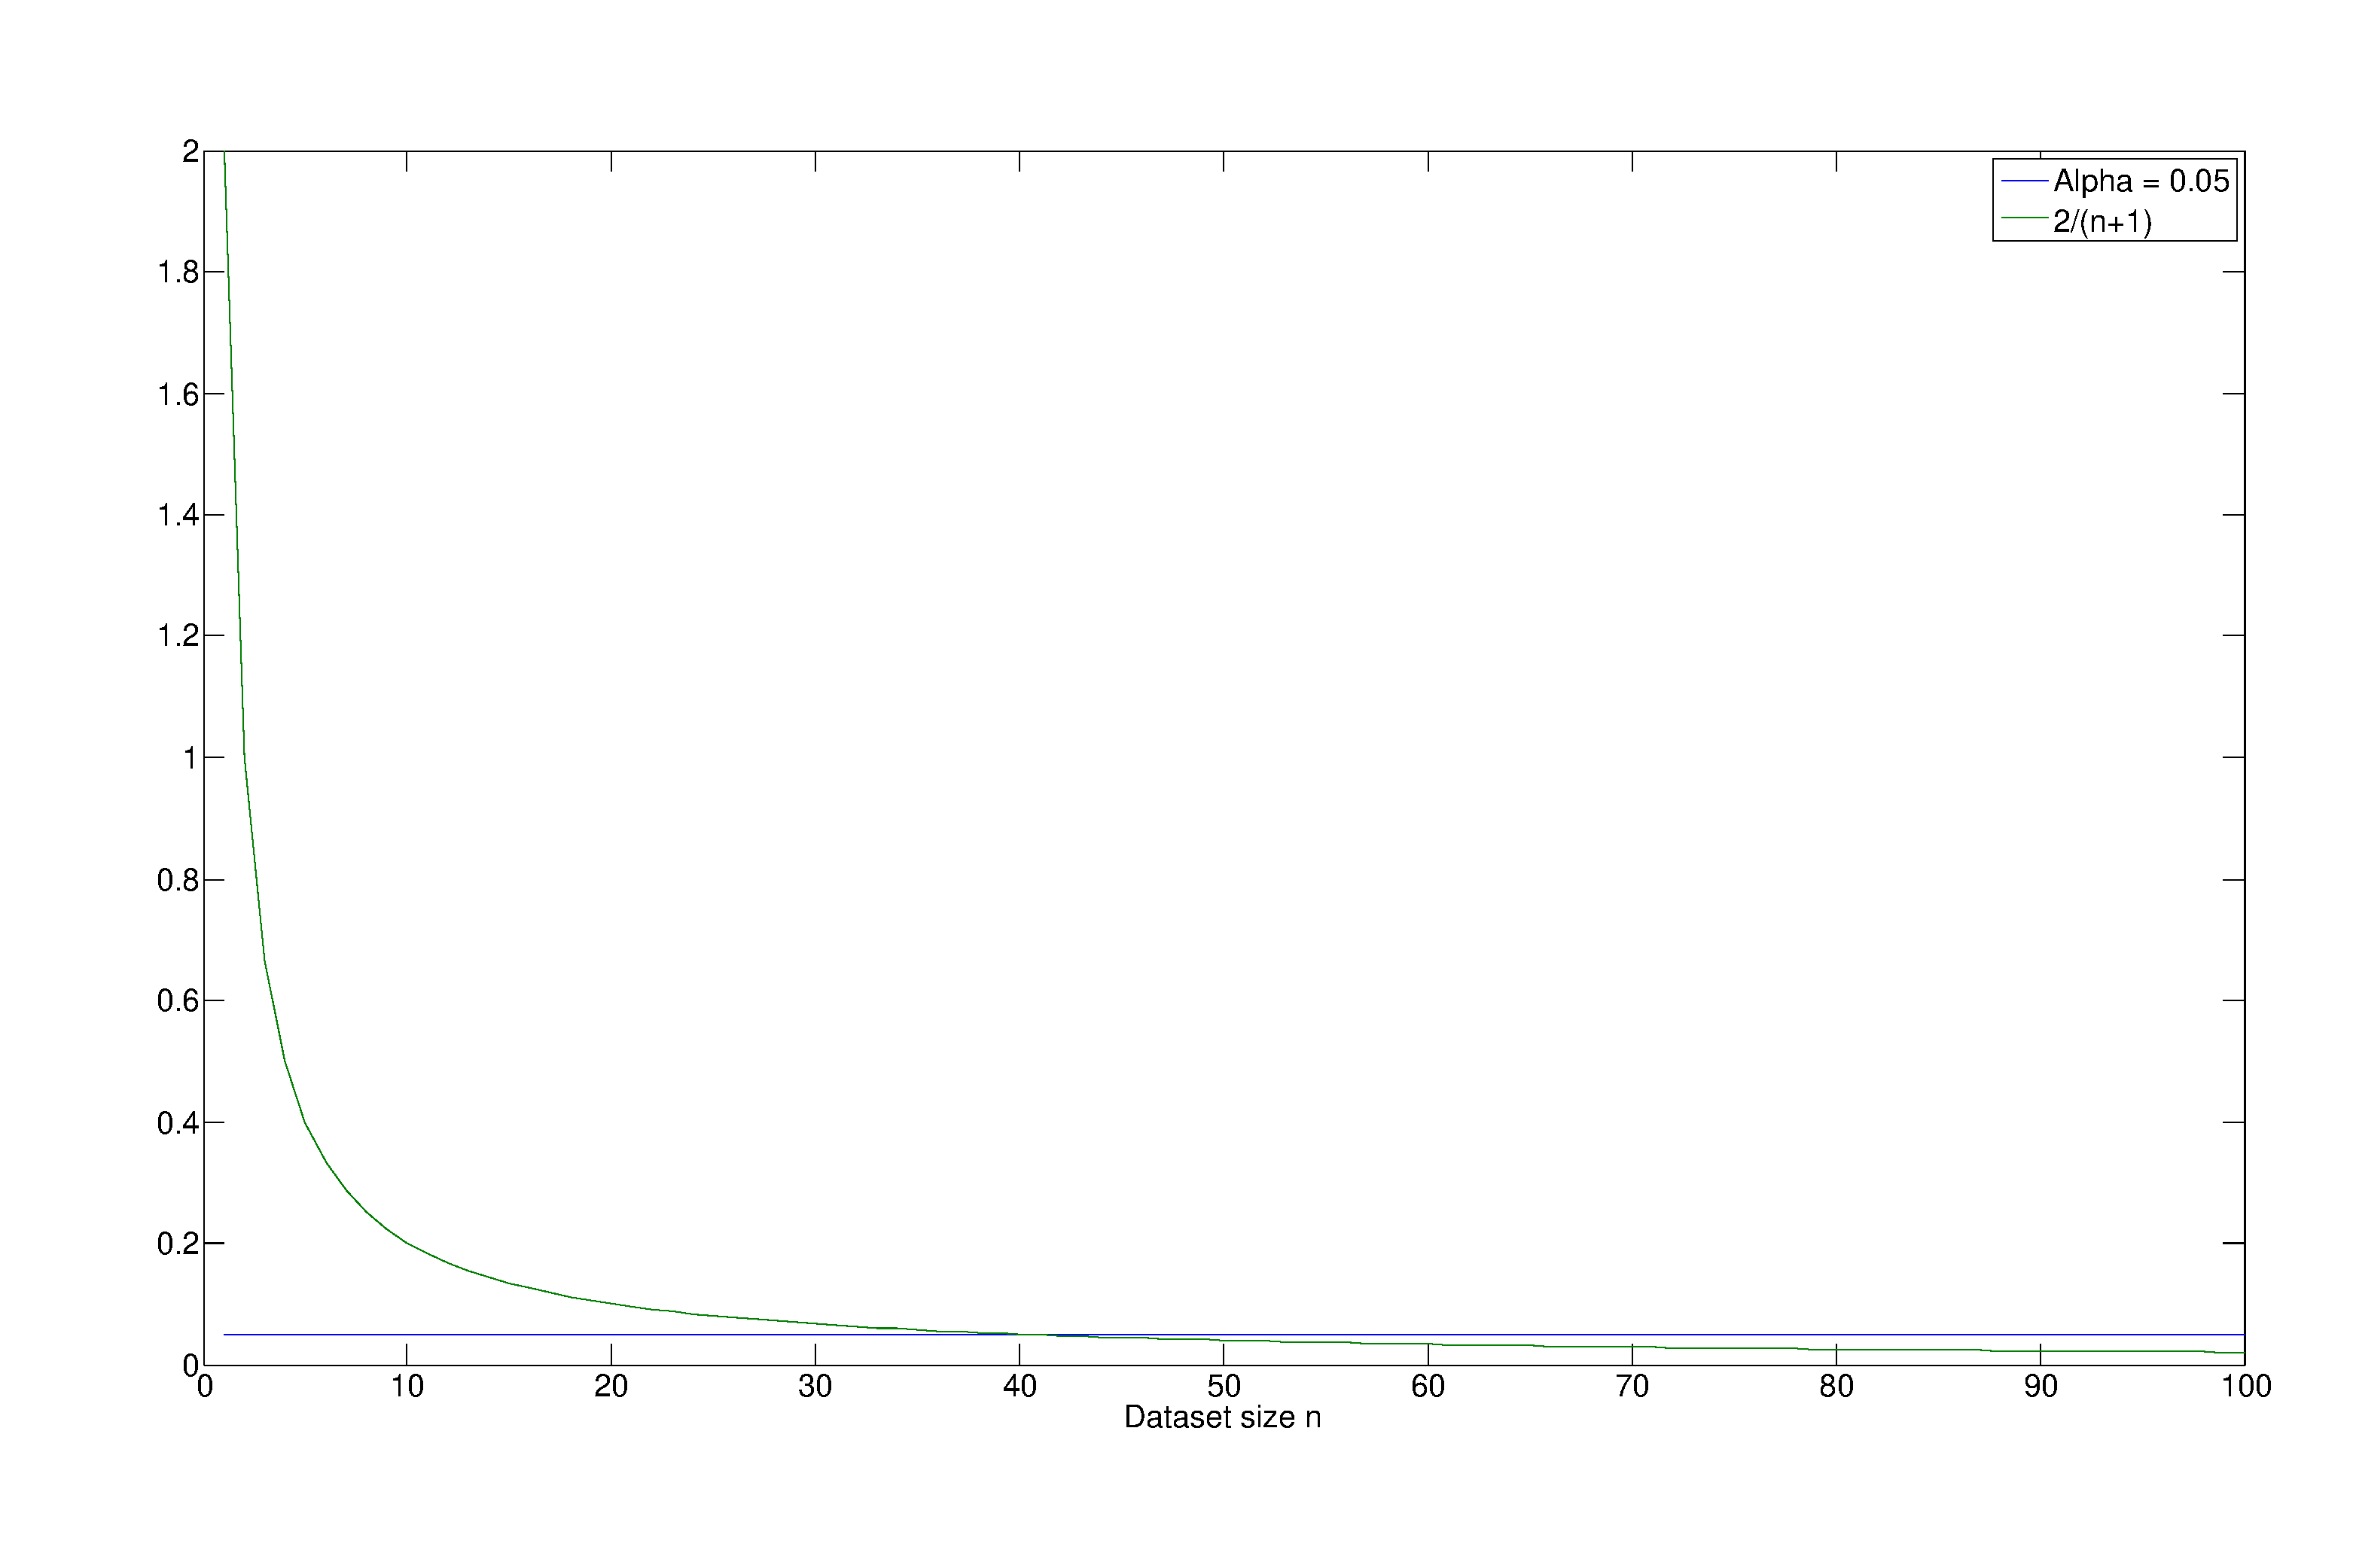
\includegraphics[width=0.6\textwidth]{images/hw1_4_d_alpha}
  \caption{Allowed dataset size $n$ for 95\% prediction interval computation with order statistic}
  \label{fig:alpha}
\end{figure}

\begin{figure}[h!]
  \centering
  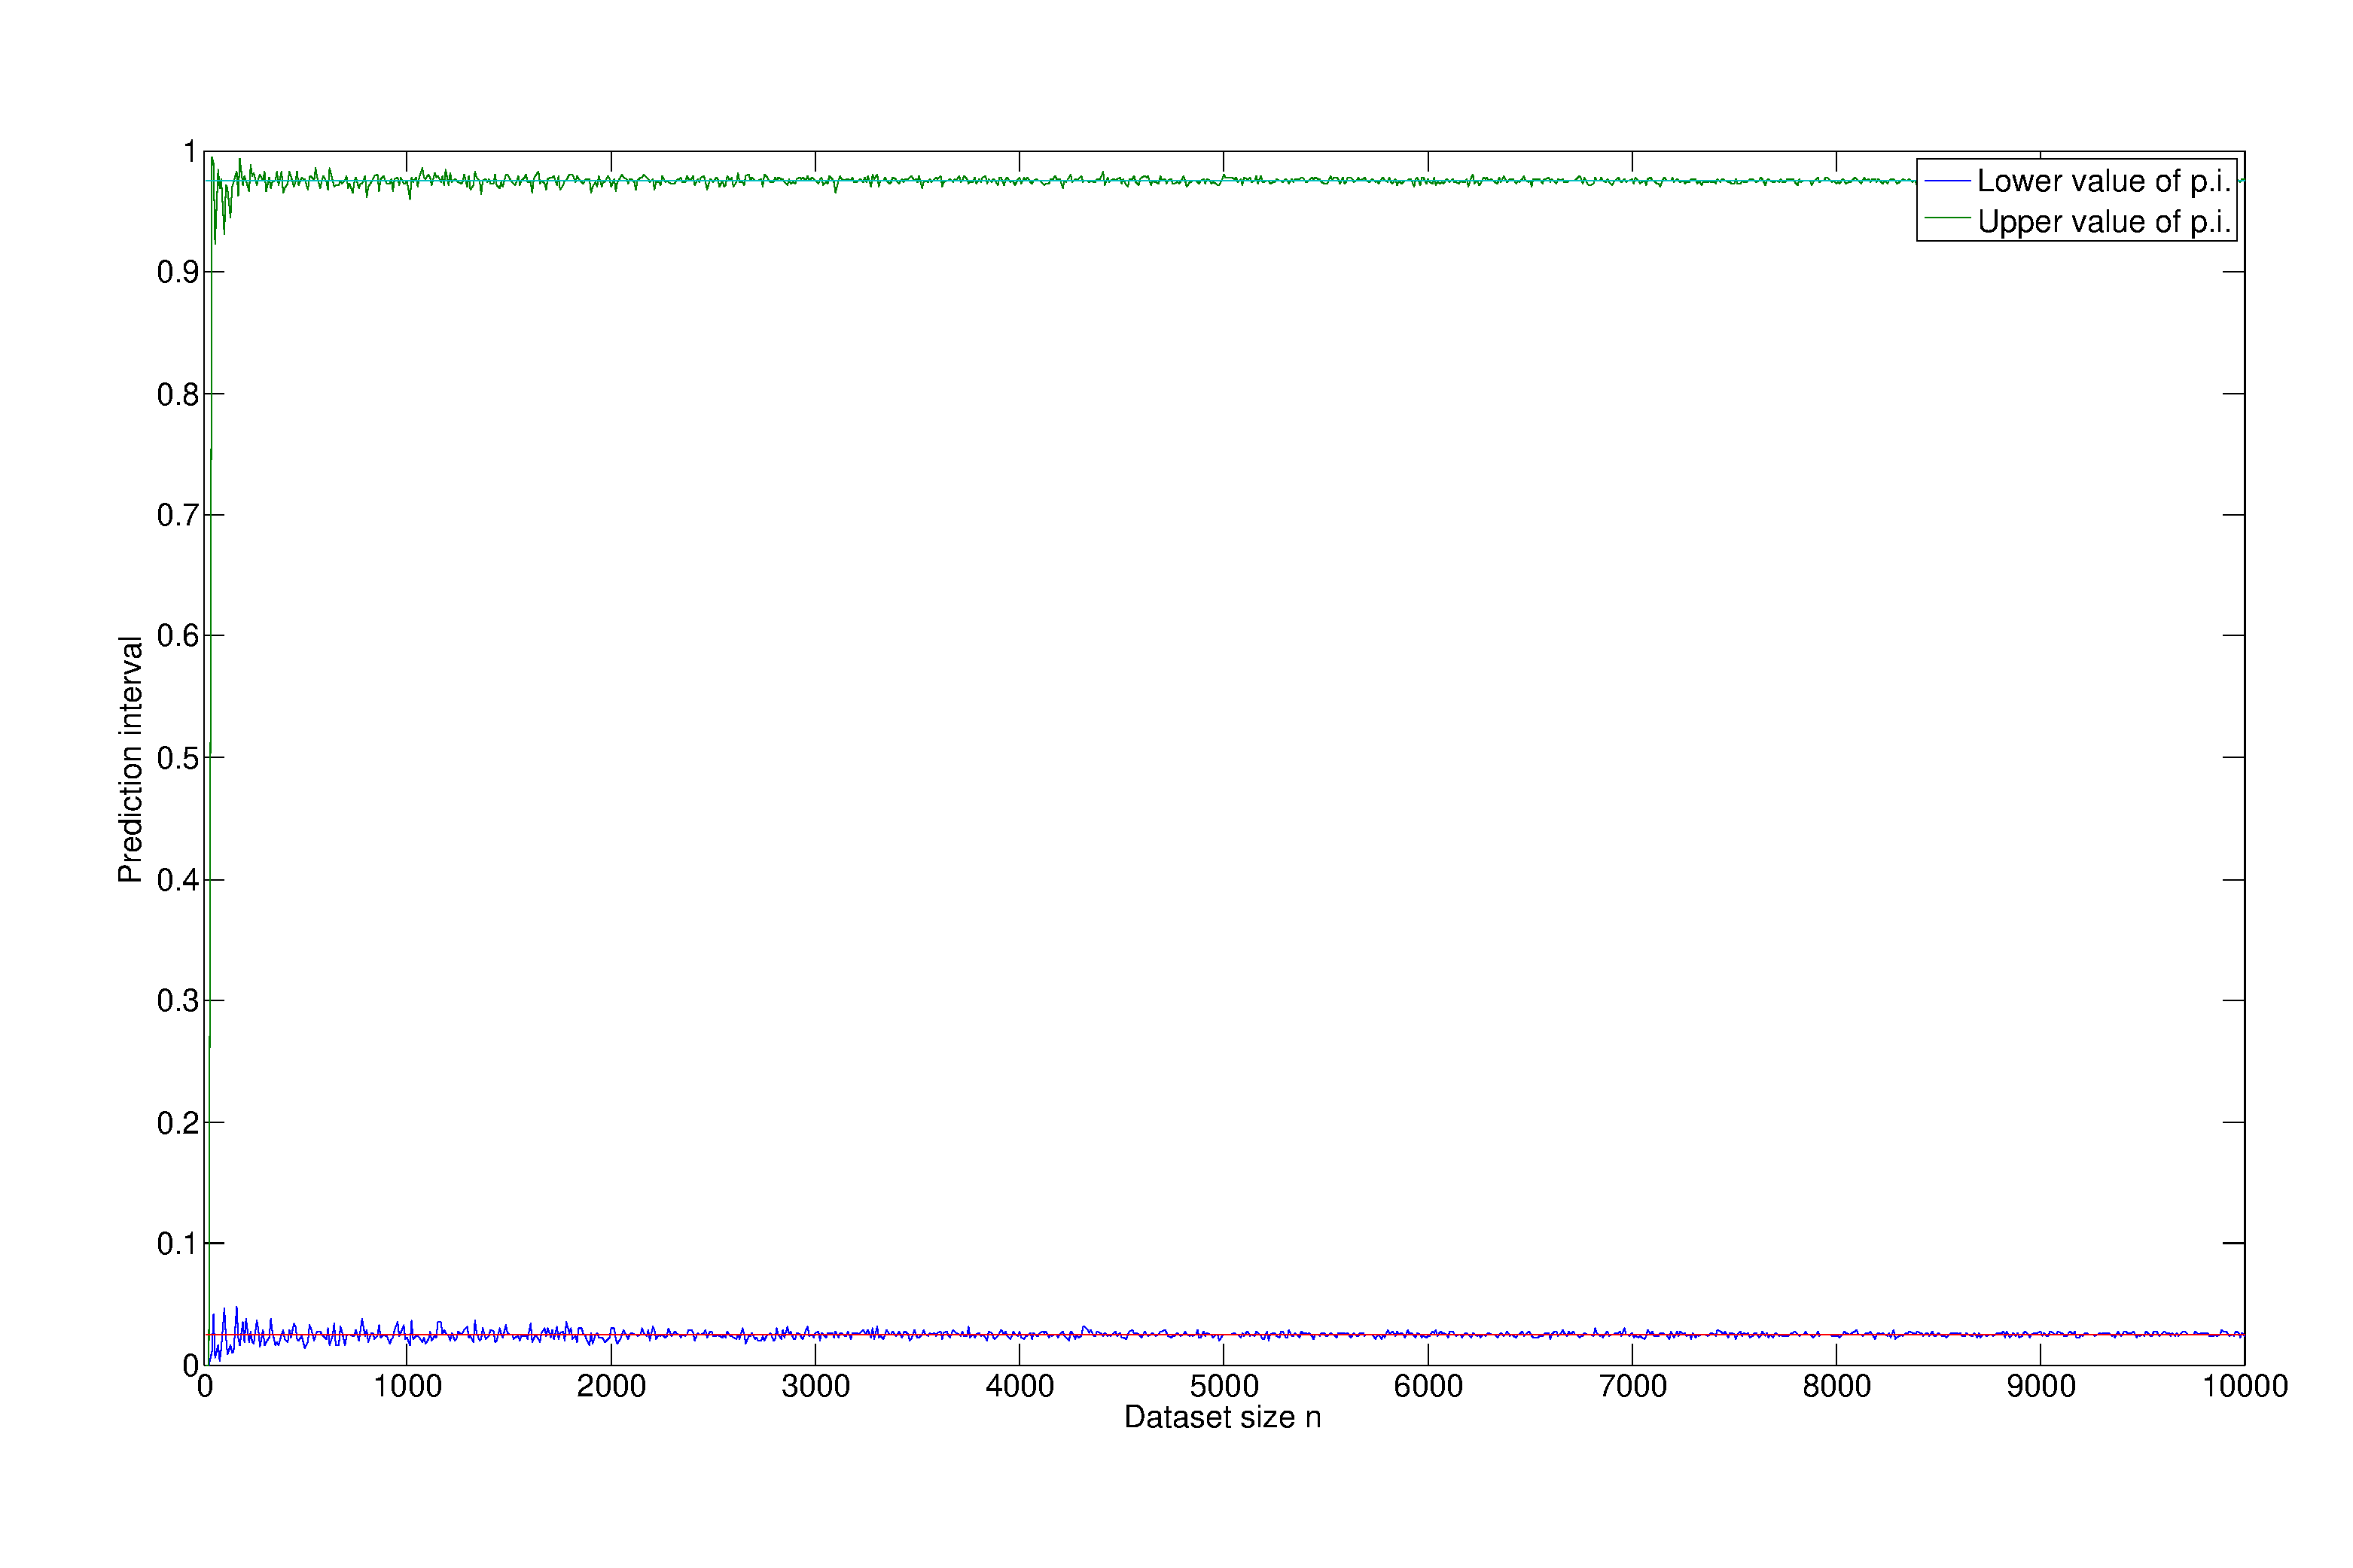
\includegraphics[width=0.6\textwidth]{images/hw1_4_d_uni}
  \caption{95\% prediction interval for a U[0,1] dataset as a function of n}
  \label{fig:pi_uni}
\end{figure}

The prediction interval can be computed also with an alternative version of the bootstrap method, described in the code below and based once again on Theorem 2.5 in \cite{leb}. However this is an approximation of the prediction interval, because Theorem 2.5 gives an exact result on the original dataset, while the bootstrap computes the same result on a resampling of the dataset. The result is in Figure~\ref{fig:pi_uni_boot}. In Figure~\ref{fig:pi_small_uni} there's a comparison between the two methods for small values of $n$.

\lstinputlisting{code/bootstrap_pi.m}

\begin{figure}[h!]
  \centering
  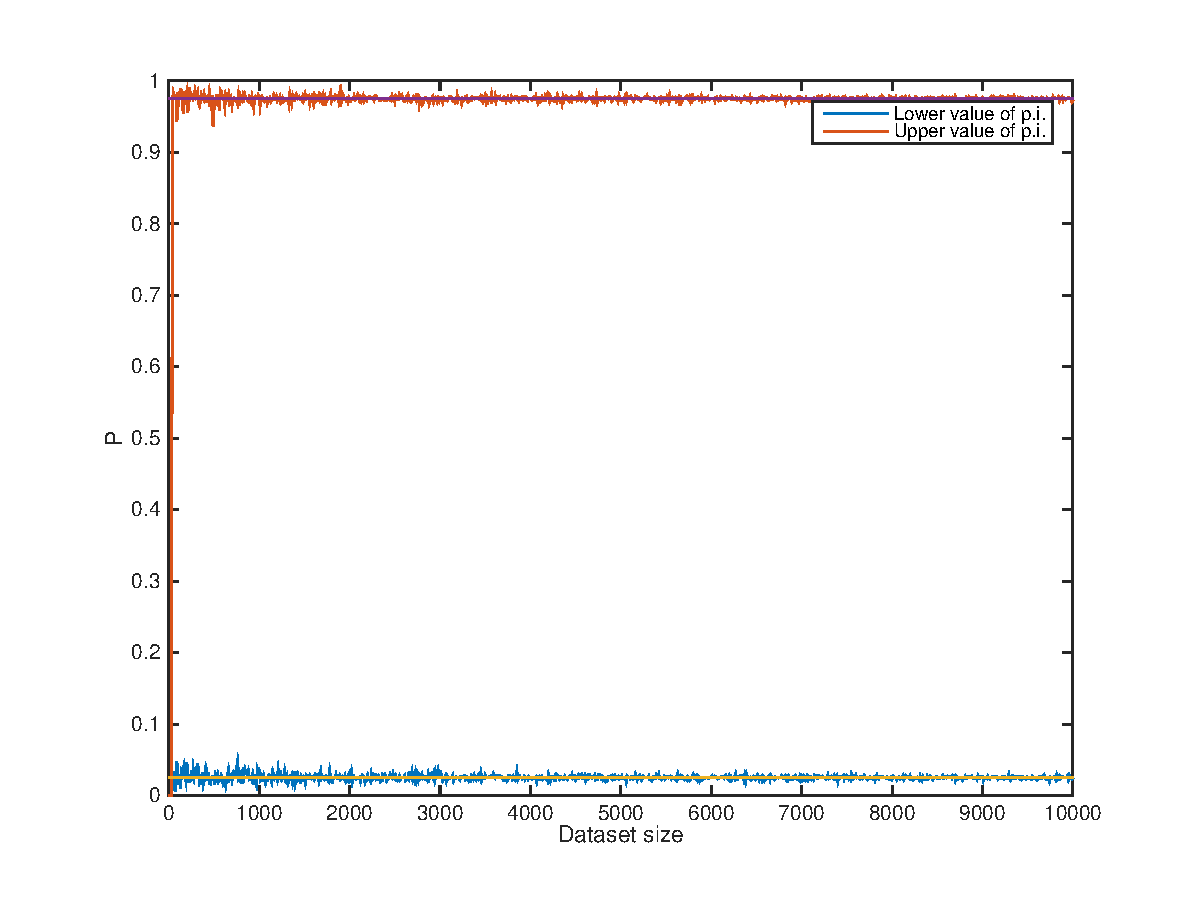
\includegraphics[width=0.6\textwidth]{images/hw1_4_d_uni_boot}
  \caption{95\% prediction interval for a U[0,1] dataset as a function of n with bootstrap method}
  \label{fig:pi_uni_boot}
\end{figure}

\clearpage

\begin{figure}[h!]
\centering
	\subfigure{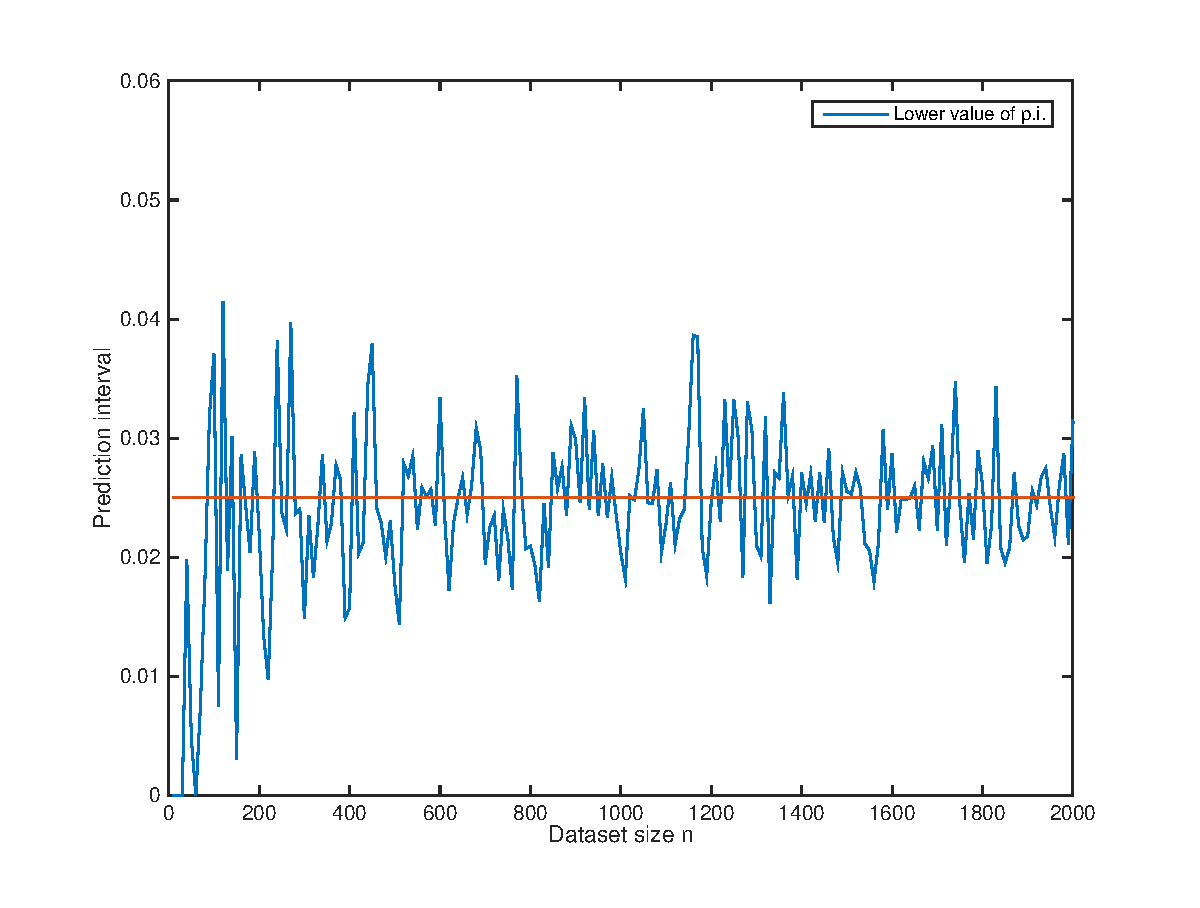
\includegraphics[width=0.45\textwidth]{images/hw1_4_d_uni_low}}
	\subfigure{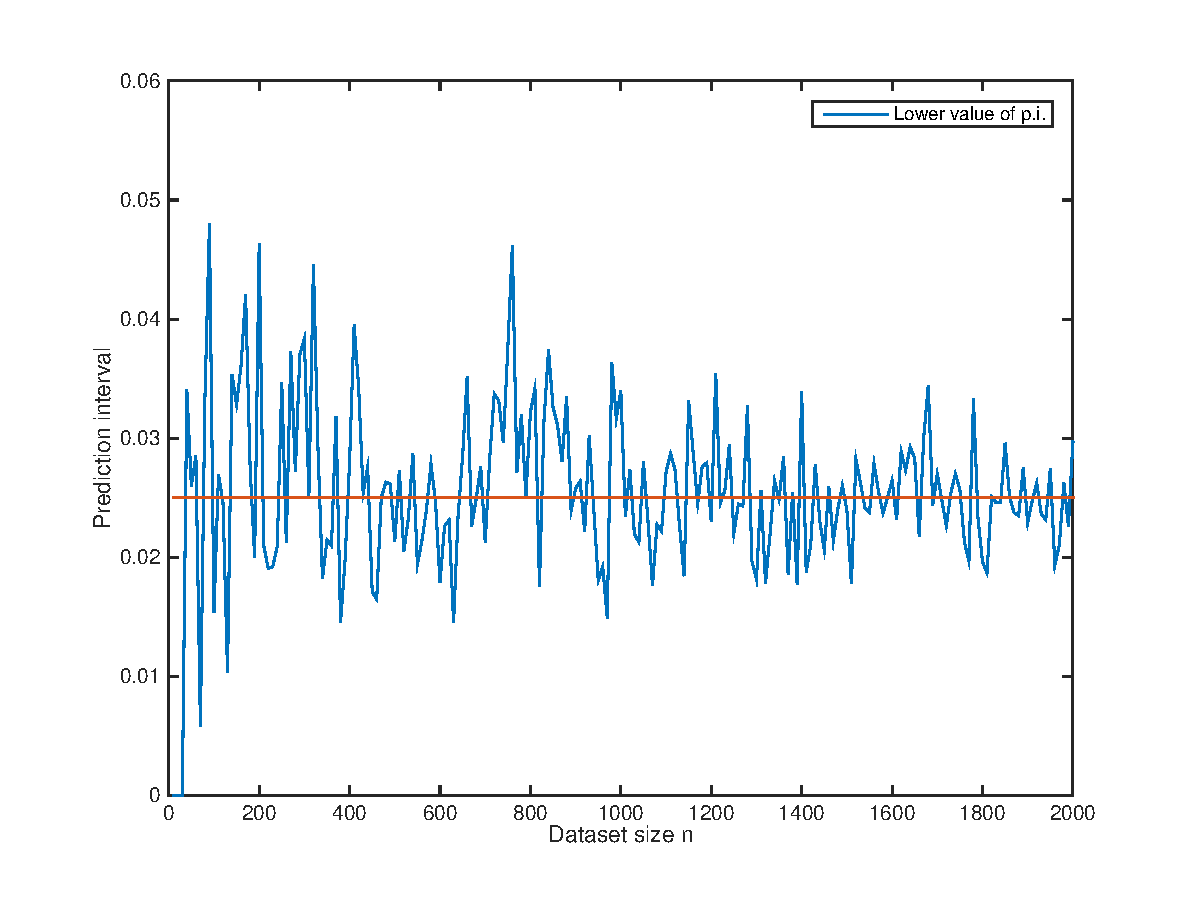
\includegraphics[width=0.45\textwidth]{images/hw1_4_d_uni_boot_low}}
 	 \caption{Lower value of prediction interval for small $n$ computed with Theorem 2.5 and bootstrap method}
  \label{fig:pi_small_uni}
\end{figure}



For iid normal $N[0,1]$ datasets instead it is possible to use another result, described in Theorem 2.6 in \cite{leb}. The 95\% prediction interval for normal dataset \{$x_1, ... , x_n$\} is $\hat{\mu}_n \pm \eta \hat{s}_n \sqrt{1 + \frac{1}{n}}$ with $\eta$ the $(1-\frac{\alpha}{2})$ quantile of $t_{n-1}$ student distribution.\\
In Figures~\ref{fig:pi_norm},~\ref{fig:pi_norm_th} and~\ref{fig:pi_norm_boot} there's a comparison between the 95\% prediction interval computed for a dataset of size $n$ with the general method, with the method for normal datasets and with bootstrap. As it can be seen in Figure~\ref{fig:pi_small_norm} the second one presents better results for small $n$, since it is based on the gaussianity of the dataset, while for larger $n$ the 3 are approximately the same. Note that formula provided by Theorem 2.6 has a weak dependence on the dataset size $n$, and for large $n$ it is approximated by $\hat{\mu}_n \pm \eta \hat{s}_n$ with $\eta$ such that $N_{0,1}(\eta) = \frac{1+\gamma}{2}$. Note also that the formula recalls the approximation for confidence interval for the mean of Theorem 2.2 in \cite{leb}, without the $\sqrt{n}$ factor that divides the standard deviation, so it doesn't change a $n$ gets larger. The grassy behavior which is present in Figure~\ref{fig:pi_norm_th} for small $n$ is due to the less accurate estimate of sample mean and sample standard deviation used to perform the calculation.

\begin{figure}[h!]
  \centering
  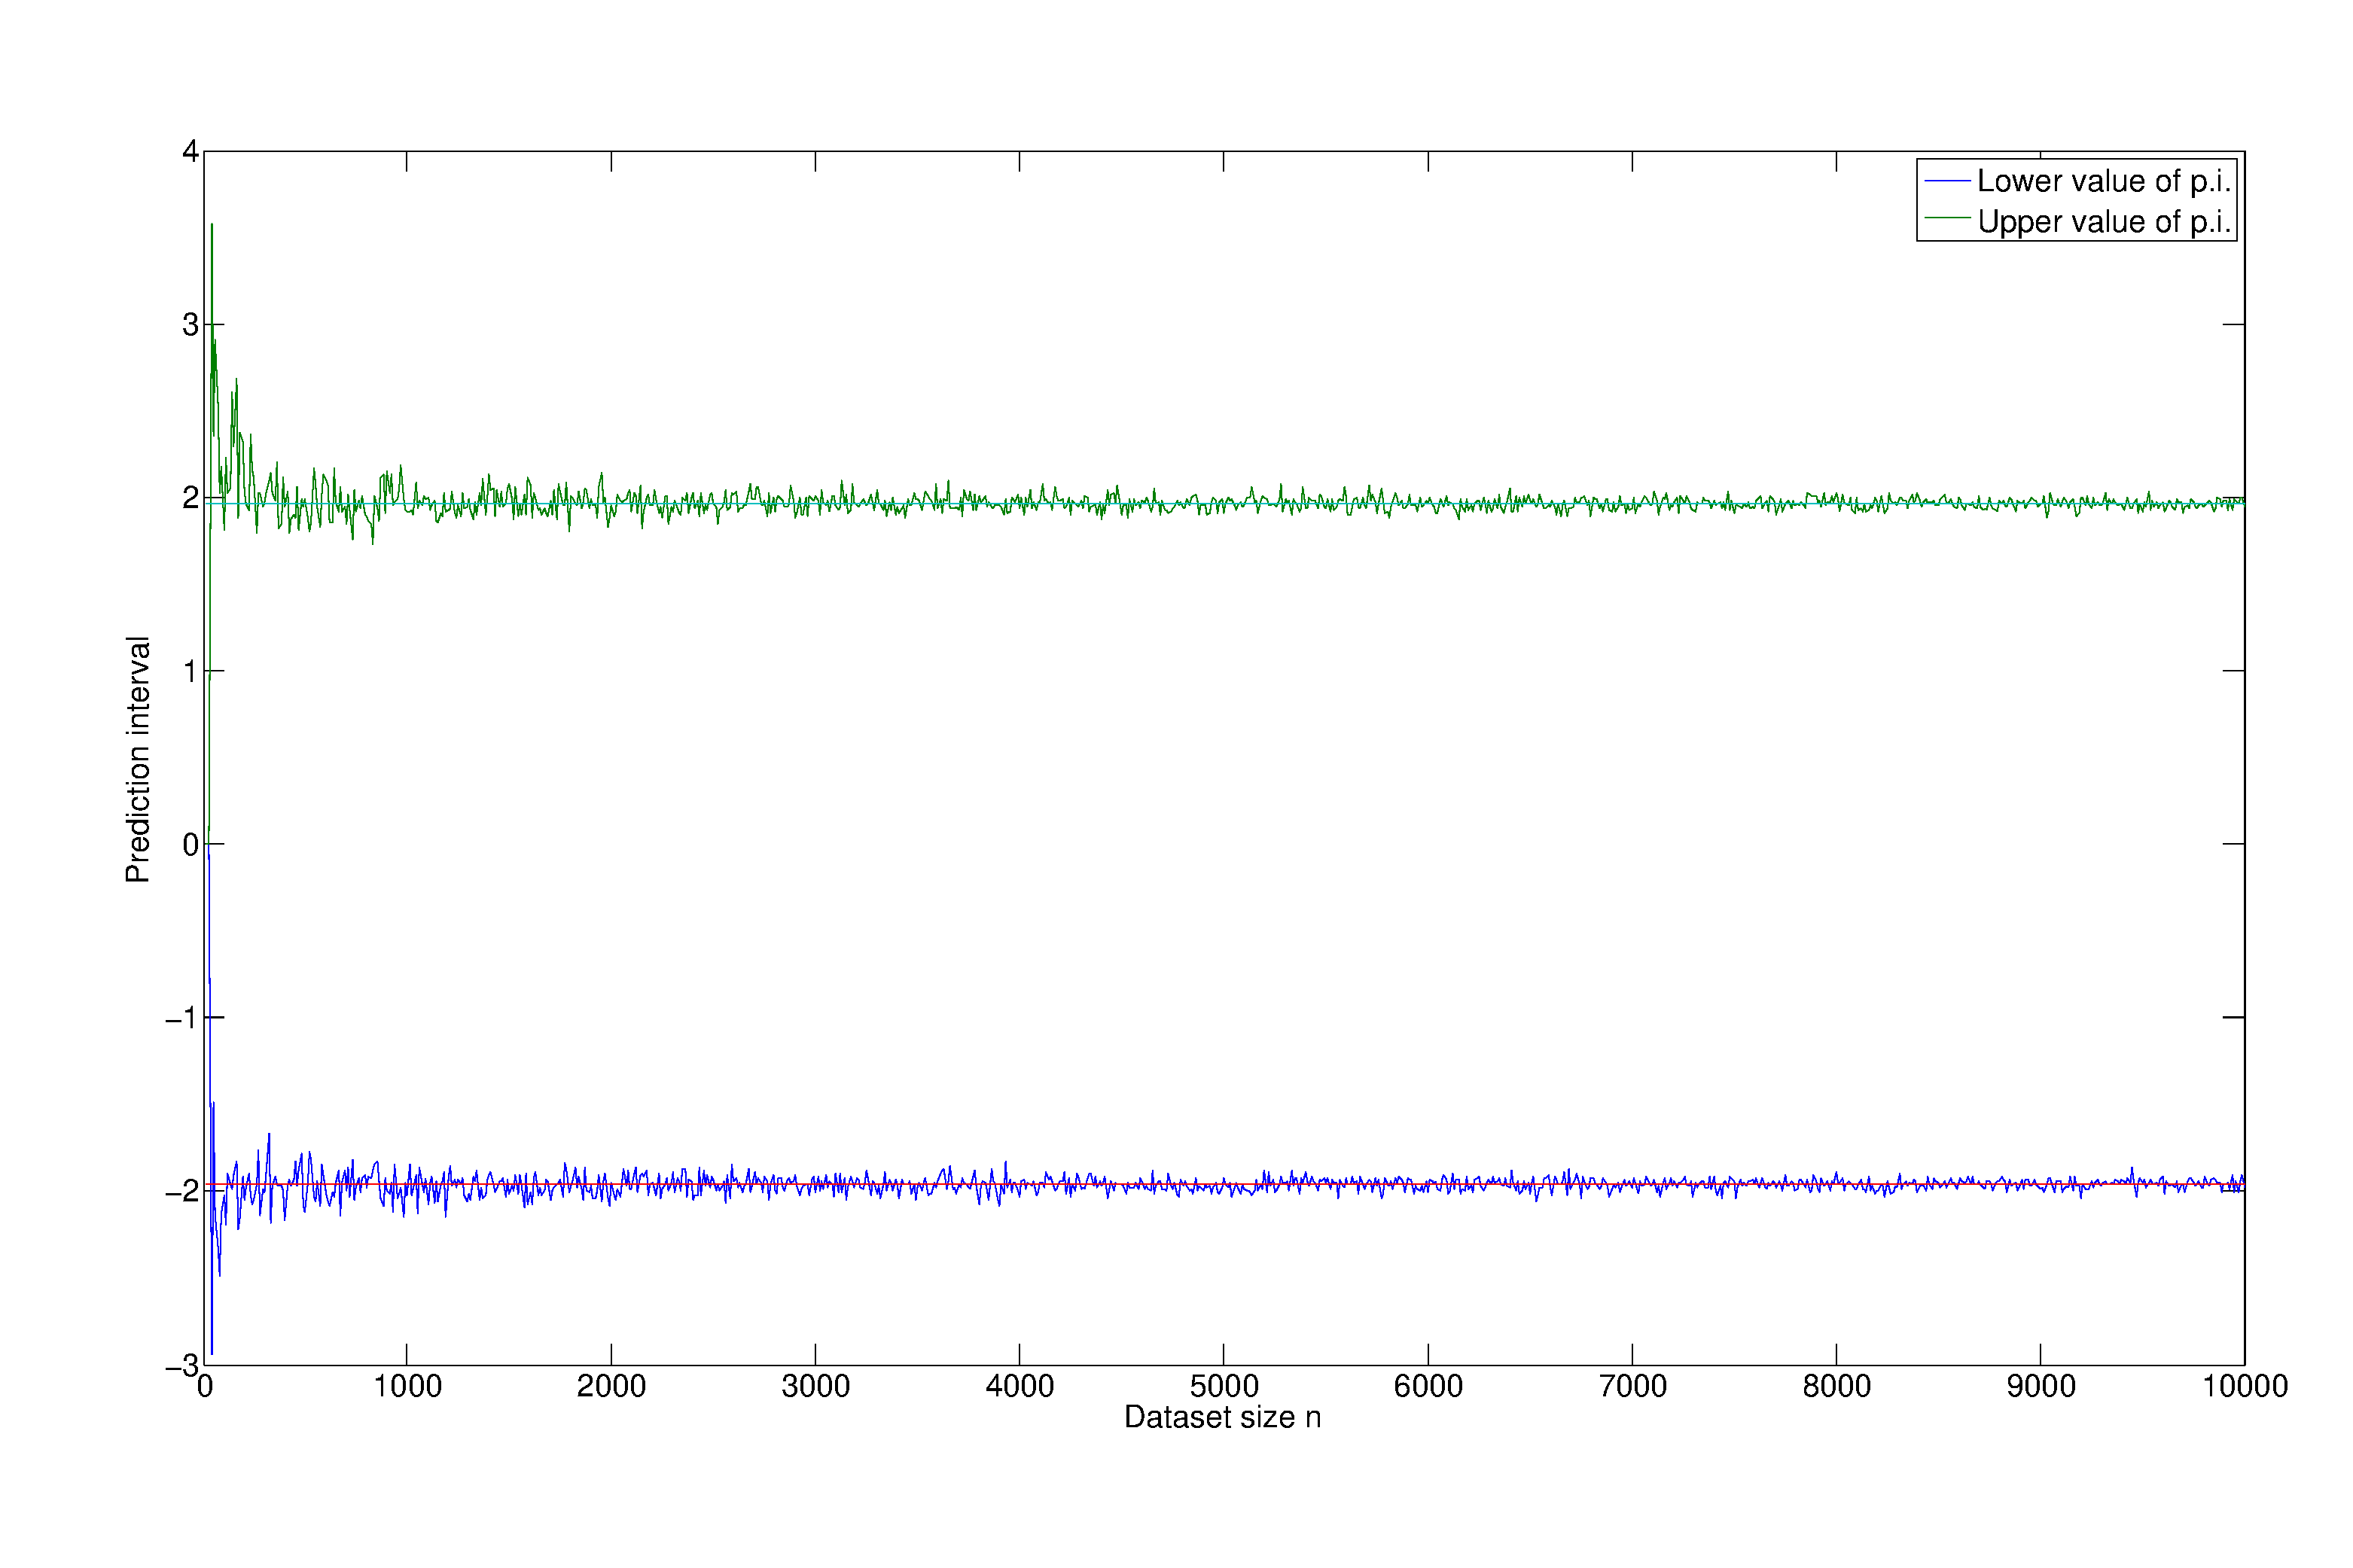
\includegraphics[width=0.6\textwidth]{images/hw1_4_d_norm_order}
  \caption{95\% prediction interval for a N[0,1] dataset as a function of n, from Theorem 2.5 in \cite{leb}}
  \label{fig:pi_norm}
\end{figure}

\begin{figure}
  \centering
  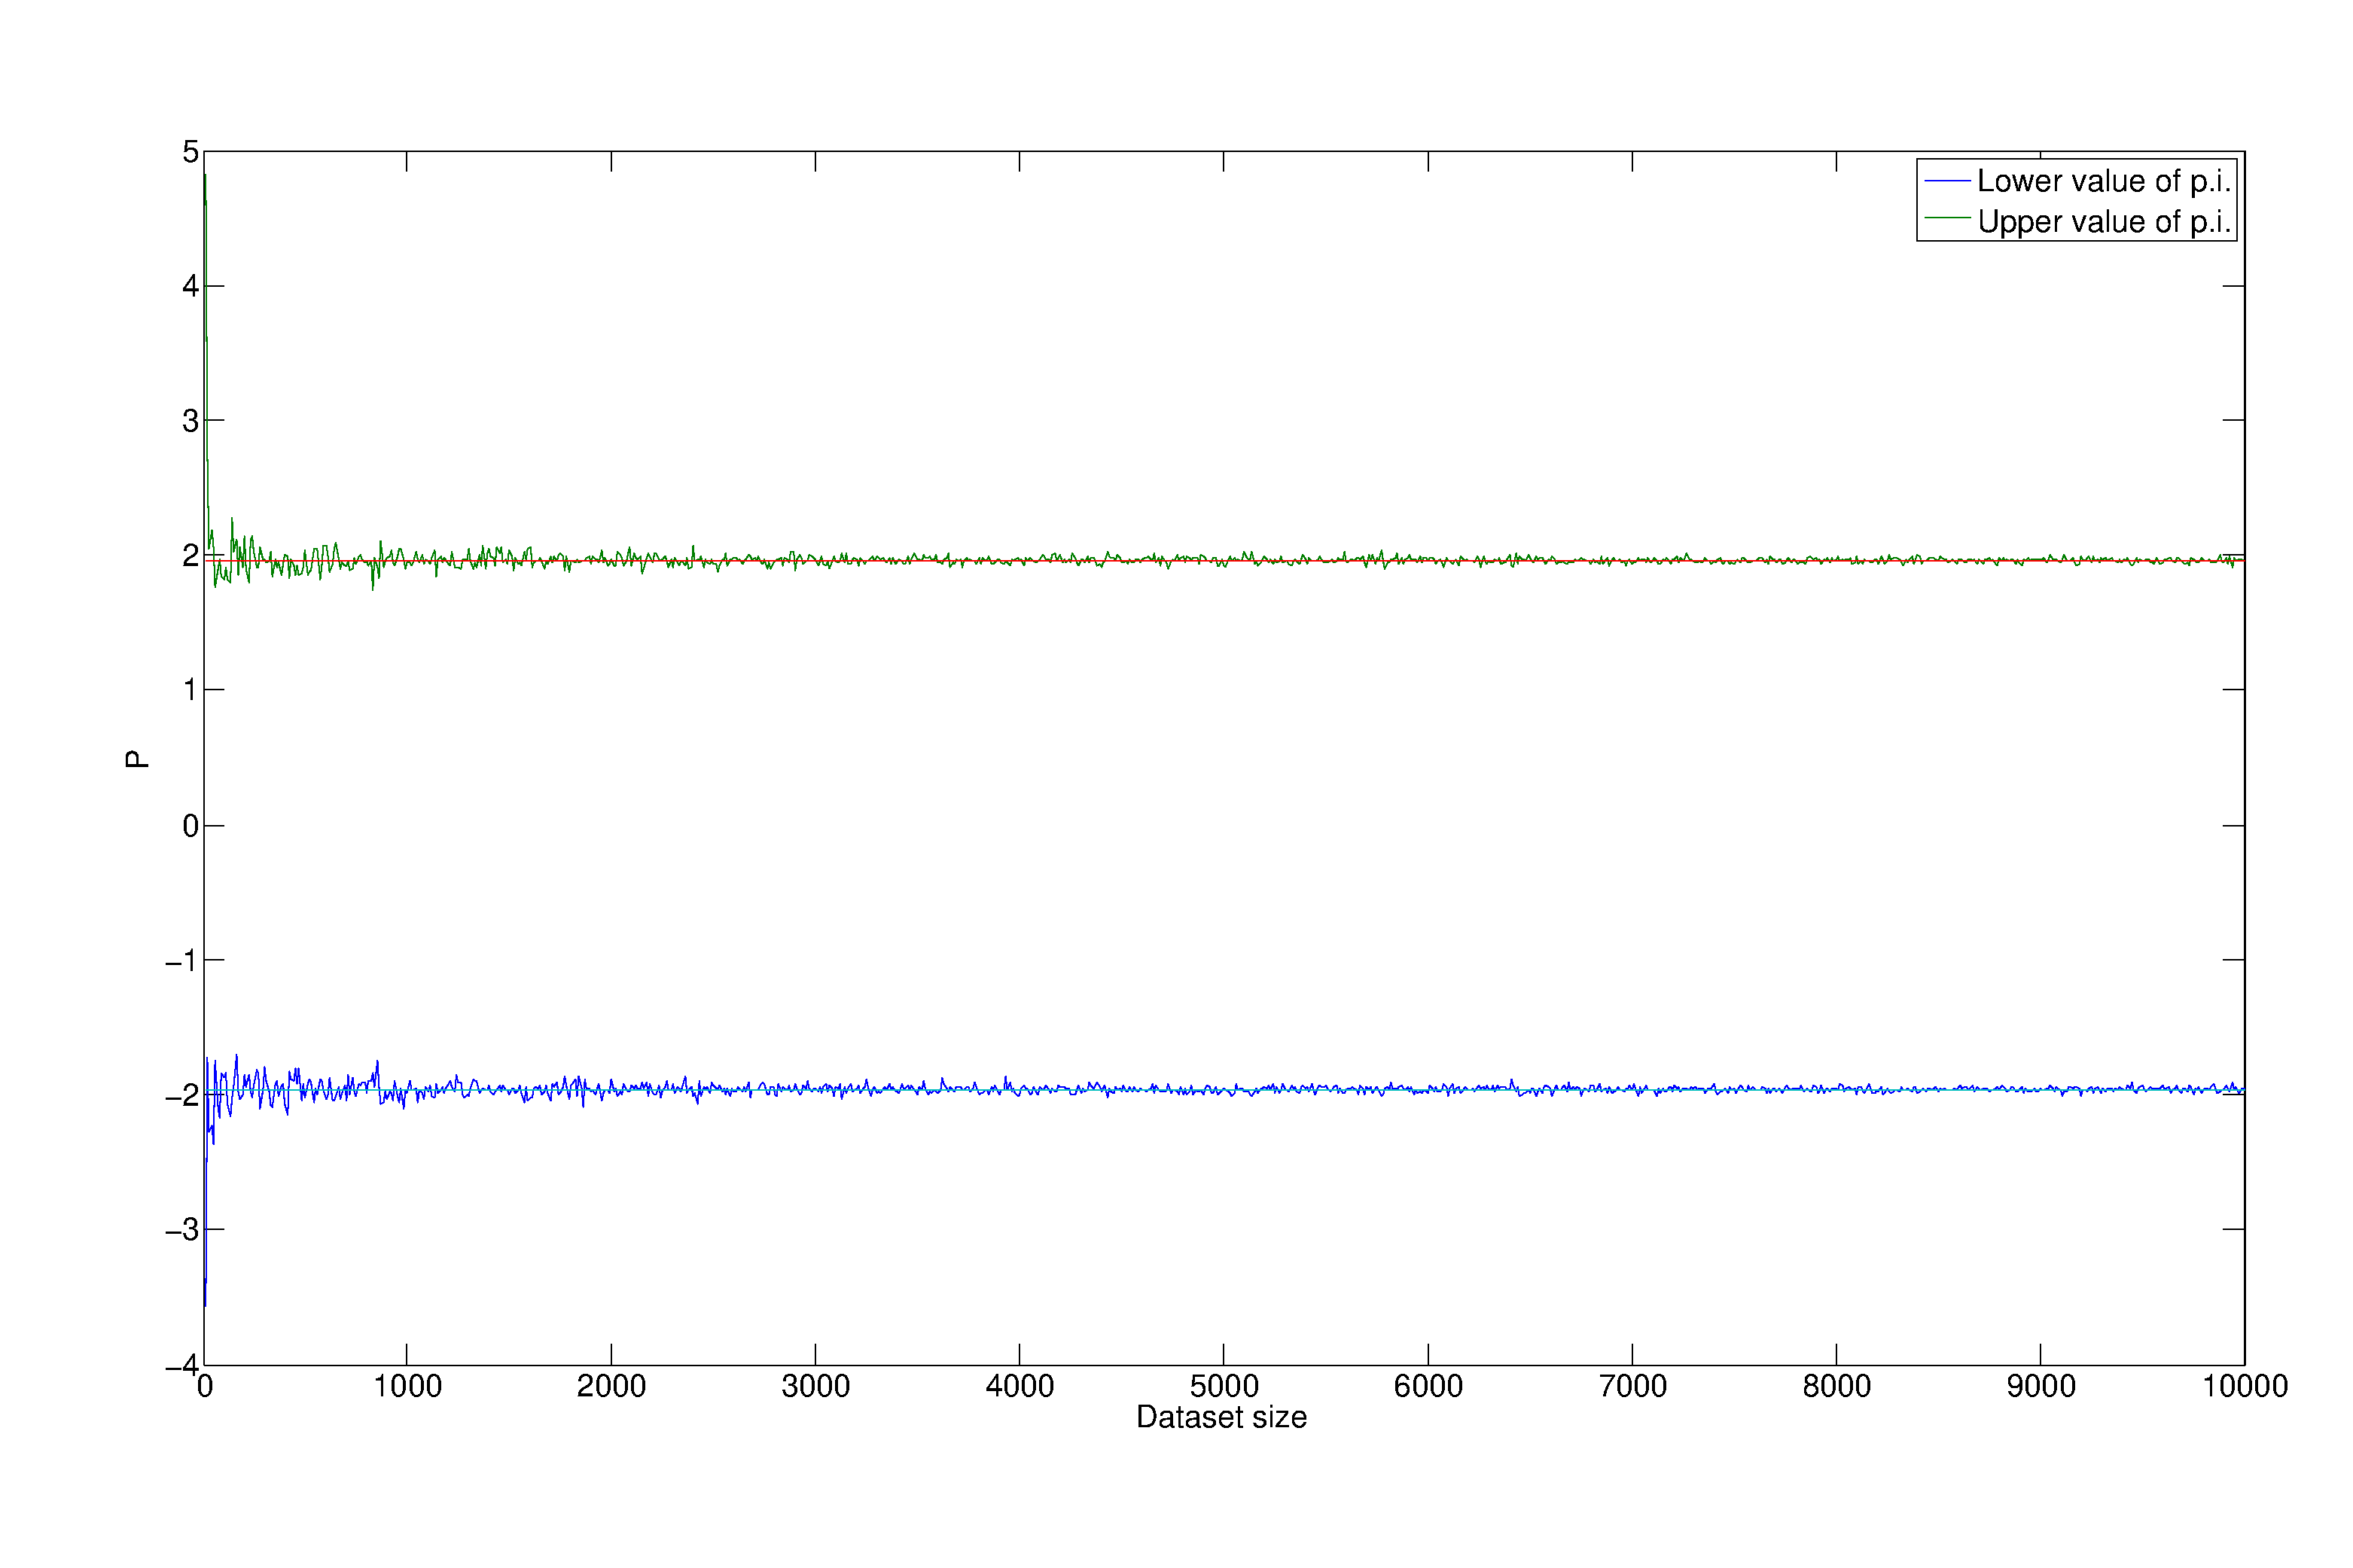
\includegraphics[width=0.6\textwidth]{images/hw1_4_d_norm}
  \caption{95\% prediction interval for a N[0,1] dataset as a function of n, from Theorem 2.6 in \cite{leb}}
  \label{fig:pi_norm_th}
\end{figure}

\begin{figure}
  \centering
  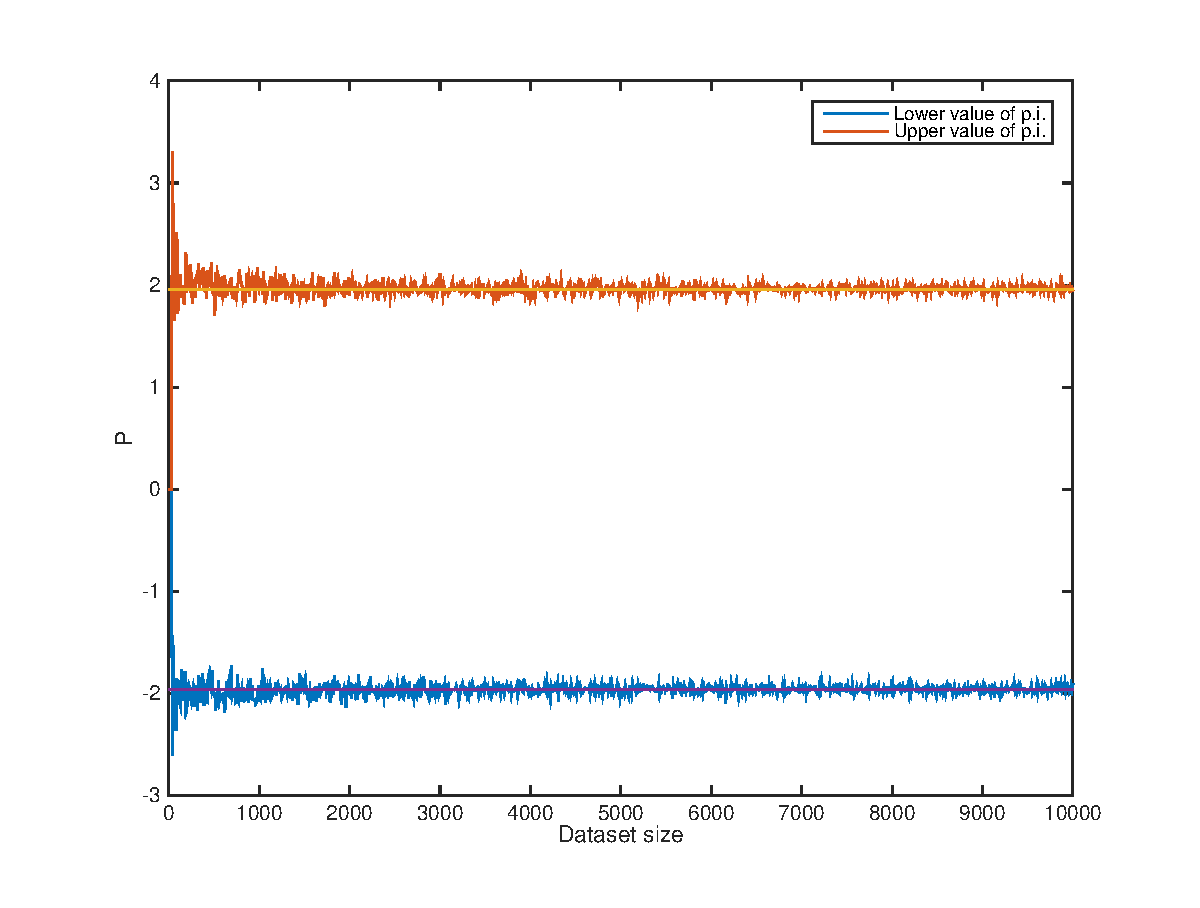
\includegraphics[width=0.6\textwidth]{images/hw1_4_d_norm_boot}
  \caption{95\% prediction interval for a N[0,1] dataset as a function of n with bootstrap method}
  \label{fig:pi_norm_boot}
\end{figure}

\begin{figure}[h!]
\centering
	\subfigure{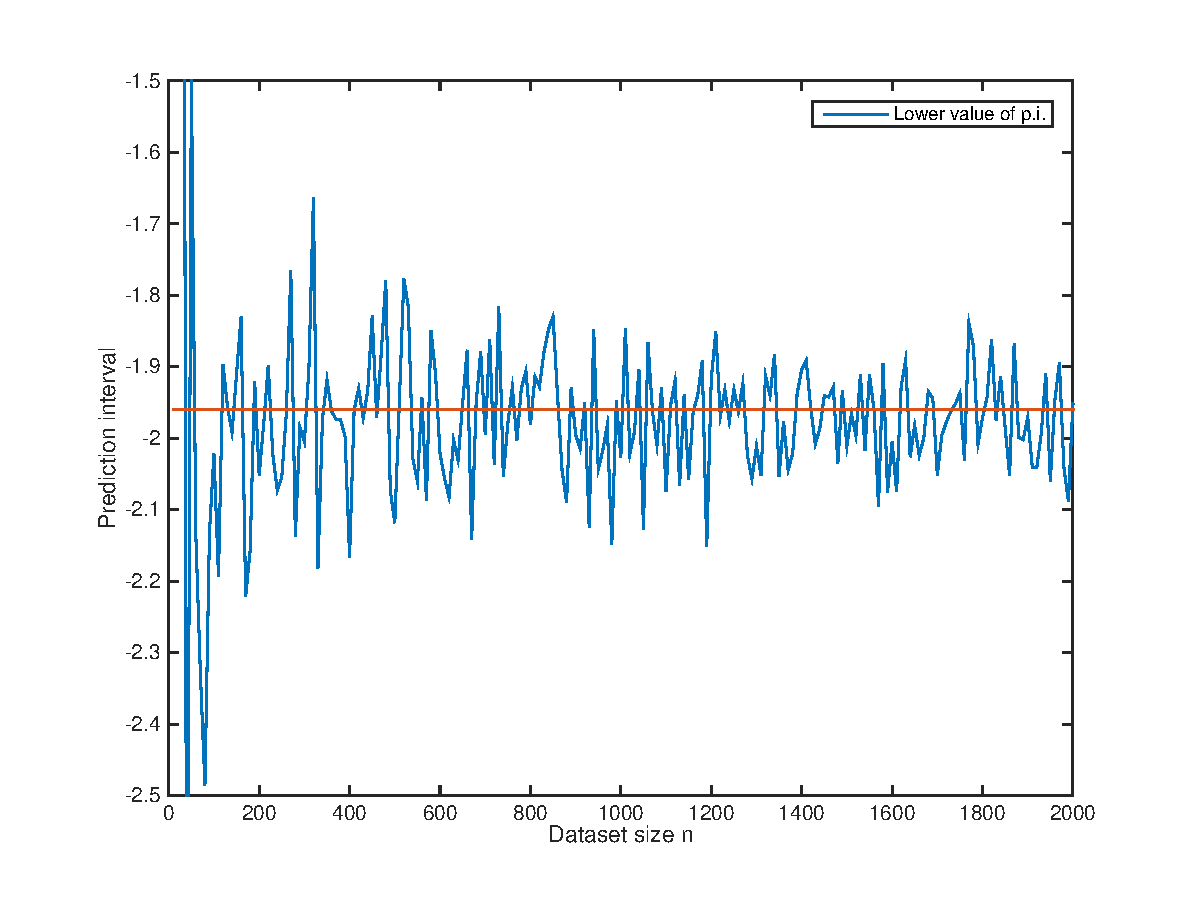
\includegraphics[width=0.45\textwidth]{images/hw1_4_d_norm_order_low}}
	\subfigure{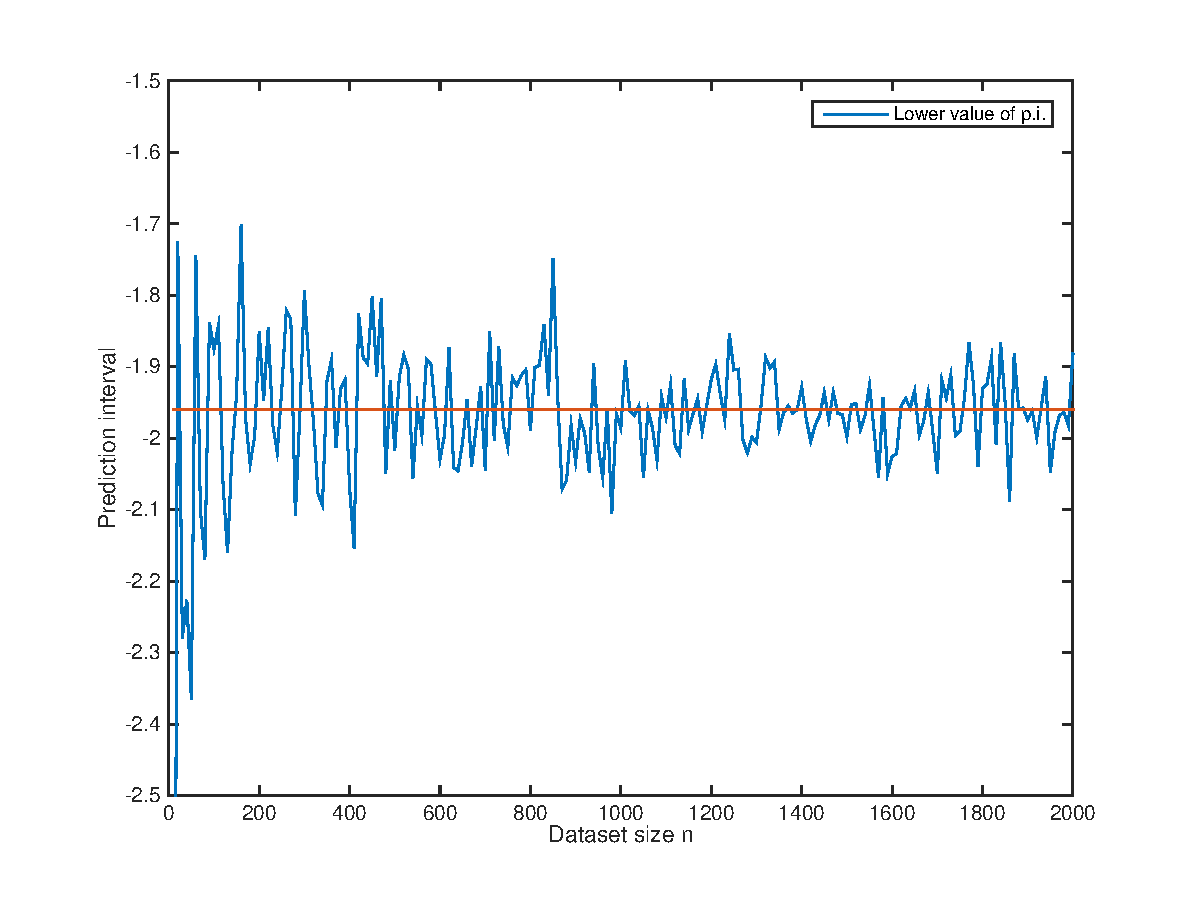
\includegraphics[width=0.45\textwidth]{images/hw1_4_d_norm_low}}
	\subfigure{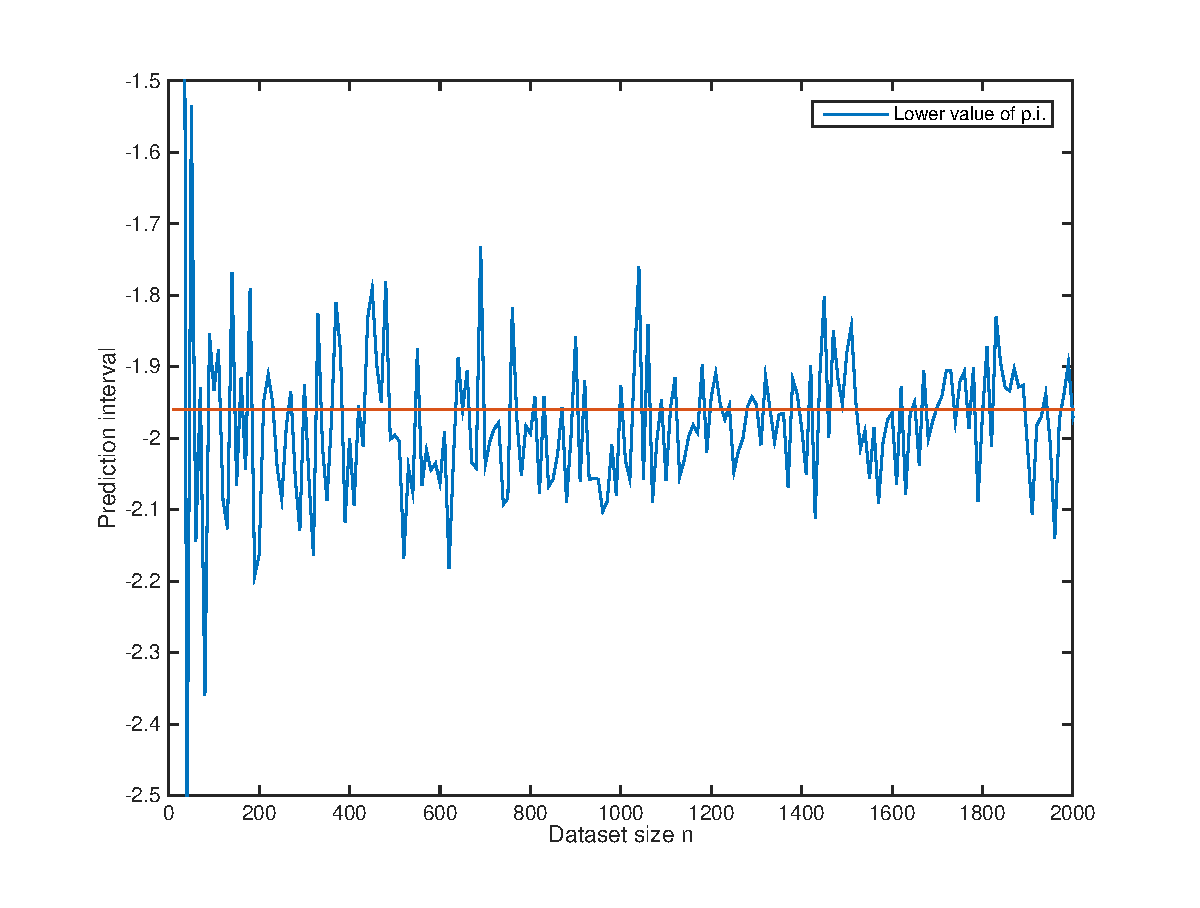
\includegraphics[width=0.45\textwidth]{images/hw1_4_d_norm_boot_low}}
 	 \caption{Lower value of prediction interval for small $n$ computed with Theorem 2.5, the exact result for normal distributions and bootstrap method}
  \label{fig:pi_small_norm}
\end{figure}


\begin{thebibliography}{10}
\expandafter\ifx\csname url\endcsname\relax
  \def\url#1{\texttt{#1}}\fi
\expandafter\ifx\csname urlprefix\endcsname\relax\def\urlprefix{URL}\fi
\expandafter\ifx\csname href\endcsname\relax
  \def\href#1#2{#2} \def\path#1{#1}\fi


\bibitem{leb}
Y. Le Boudec, Performance Evaluation of Computer and Communications Systems, EPFL, 2015

\bibitem{pk}
M. Pinsky, S. Karlin, An Introduction to Stochastic Modeling, $4^{th}$ edition, Elsevier, 2011


\end{thebibliography}

\end{document}
